\section{Classical Force Fields on All-Atom Proteins}
\label{sec:classical_ff}
We demonstrate that our OM action optimization framework is broadly useful for transition path sampling even beyond the setting of generative modeling. Specifically, we aim to find all-atom transition paths between the unfolded and folded states of the protein Chignolin and Trp-Cage, using a differentiable PyTorch implementation \cite{doerr2020torchmd, sipka2023differentiable} of the Amber \textit{ff14SB}\cite{14amber} forcefield and the \textit{TIP3P} implicit water model. We choose the physical parameters of the OM action to be consistent with commonly used values in molecular simulations (see Table \ref{tab:om_optimization_details_classical}). Since we do not have a generative model from which to obtain an initial path guess via latent interpolation as described in $\ref{sec:main_method}$, we instead employ a \textbf{hierarchical unwrapping} warm-up procedure described in the Appendix \ref{ape:guesses} to obtain initial paths. As the classical force field is dominated by quadratic terms whose Laplacian is constant and thus uninformative for optimization, we use a zero-temperature approximation and optimize with the Truncated OM action. Using the Truncated action, we obtain a physical transition path of length 2.6ps (shown in \fref{fig:all_atom_proteins}). This is much lower than previously reported transition path lengths for Chignolin \cite{chignolinanalysis, lindorff2011fast}, which can be explained by the fact that our trajectories proceed between the target states without fluctuations that would occur in unbiased simulations. The entire optimization took on the order of hours on one NVIDIA RTX A6000 GPU, including the generation of initial trajectory. 

\begin{figure*}[h]
    \centering
    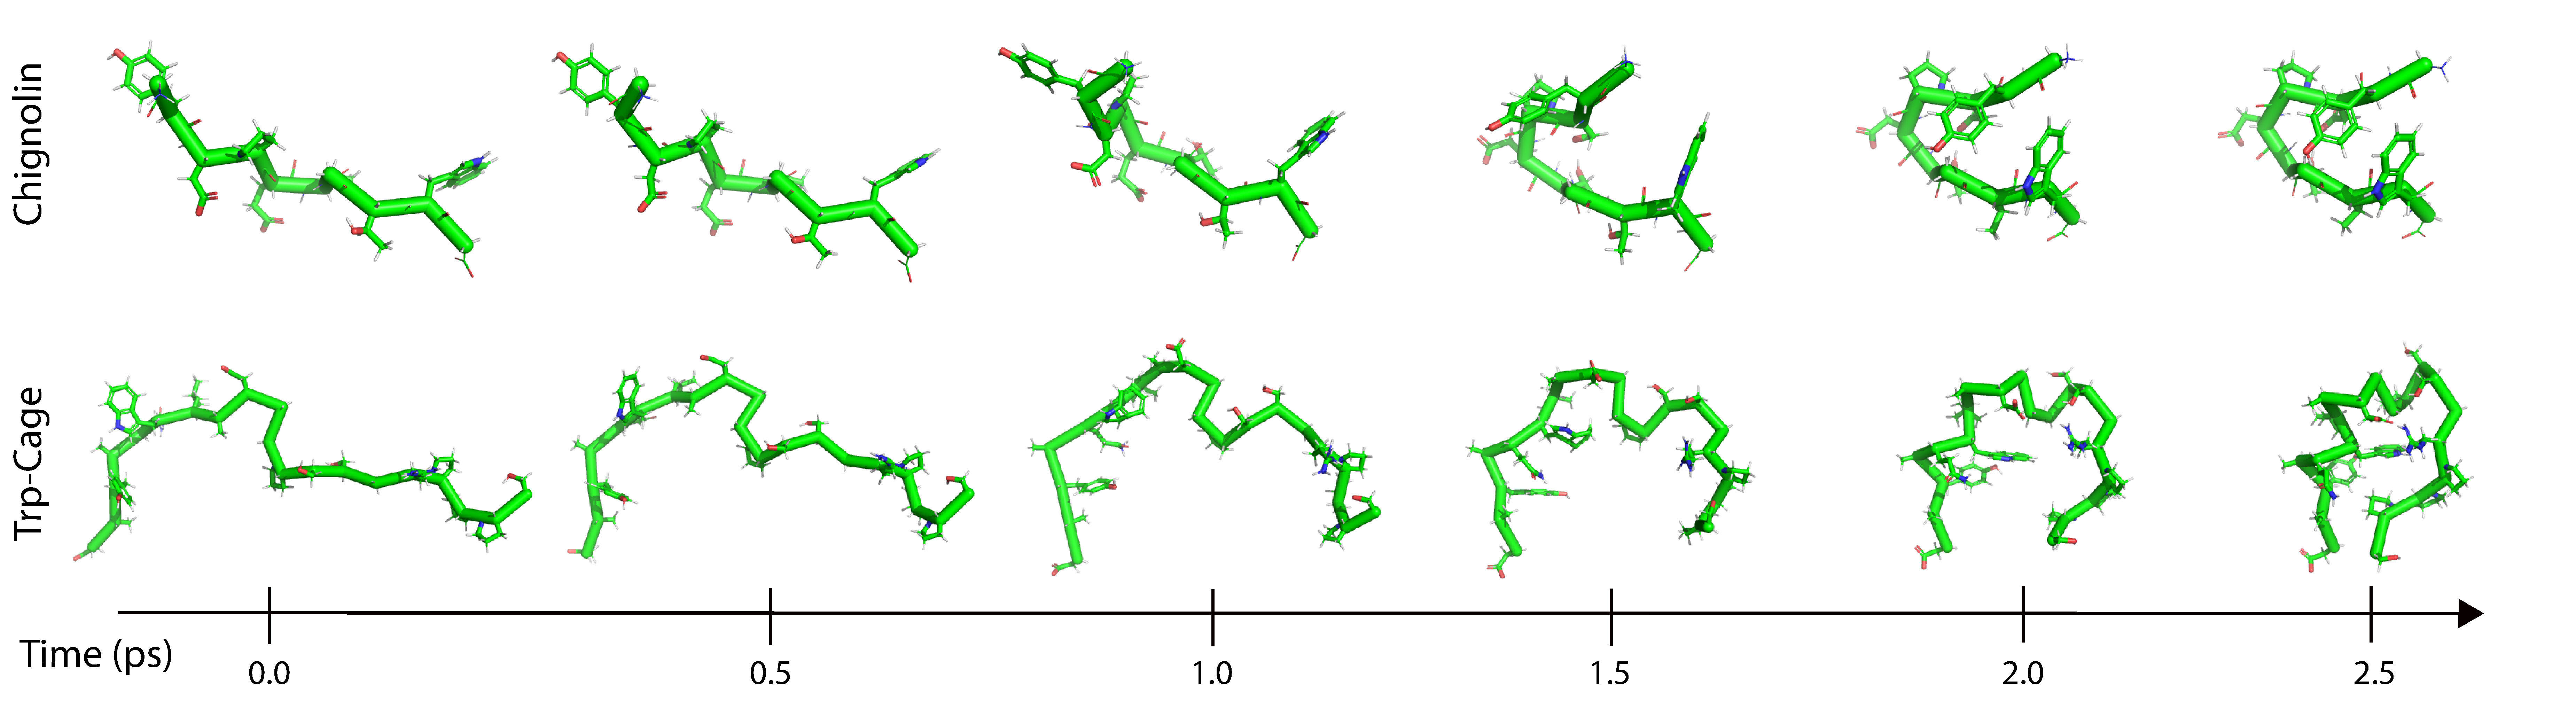
\includegraphics[width=\linewidth]{Figures/all_atom_proteins.pdf}
    \caption{Transition paths from OM optimization of all-atom chignolin and trp-cage with a classical force field.}
    \label{fig:all_atom_proteins}
\end{figure*}


\begin{table}[h]
\caption{Hyperparameters used for OM action optimization on all atom proteins}
\label{tab:om_optimization_details_classical}
\scriptsize
\centering
    \begin{tabular}{lcccc}
        \toprule
        \textbf{Hyperparameter} & \textbf{Chignolin - warmup} & \textbf{Chignolin} & \textbf{TRP Cage - warmup} & \textbf{TRP Cage} \\
        \midrule
        Number of points per path & 40 - 2600 & 2600 & 40 - 2600 & 2600 \\
        Action Type & Truncated & Truncated & Truncated & Truncated \\
        Optimizer & Adam & Adam & Adam & Adam \\
        Learning Rate & $10^{-4}$ & $10^{-5}$ & $10^{-4}$ & $10^{-5}$ \\
        Action Timestep ($\Delta t$) & $1$ fs & $1$ fs & $1$ fs & $1$ fs \\
        Action Friction ($\gamma$) & $10$ ps$^{-1}$ & $10$ ps$^{-1}$ & $10$ ps$^{-1}$ & $10$ ps$^{-1}$ \\
        \bottomrule
    \end{tabular}
\end{table}

\section{Additional Details on Onsager-Machlup Action Minimization Method}
\label{sec:om_details}


\paragraph{Initial Path Guess Methods.}
\label{ape:guesses}
We provide a complete description and algorithmic formulation of the initial path guess method using a generative model, mentioned in Section \ref{sec:main_method}.

Formally, consider a generative model with a non-parametric, probabilistic encoding (i.e corruption) process $q(\xx_\tau | \xx_0)$, and a corresponding, parametric decoding (i.e generative) process $p_\theta(\xx_0 | \xx_\tau)$. We first roto-translationally align the endpoints of the path via a Kabsch alignment \cite {kabsch1993automatic}. We encode the aligned endpoints of the path into the chosen latent level for the initial guess, $\tau_{\text{initial}}$ to produce two latent endpoints $\mathbf{z}^{(0)} \sim q(\mathbf{z}_{\tau_{\text{initial}}} | \xx^{(0)})$ and $\mathbf{z}^{(L)} \sim q(\mathbf{z}_{\tau_{\text{initial}}} | \xx^{(L)})$. We then interpolate linearly to generate a latent path $\mathbf{Z} = \left \{ \mathbf{z}^{(i)} = (1-\frac{i}{L})\mathbf{z}^{(0)} + \frac{i}{L}\mathbf{z}^{(L)} \right \}_{i \in \left[0, L \right]}$. We can then either decode the path back to the configurational space via $p_\theta(\xx | \mathbf{z}^{(i)})$ to obtain a path $\xx$, in which case the subsequent OM optimization would occur in configurational space, or defer decoding, in which case optimization occurs at the latent level $\tau_{\text{initial}}$ starting from the latent path $\mathbf{Z}$. Intuitively, larger values of $\tau_\text{initial}$ produce more diverse initial guesses at the expense of decreasing correspondence to the endpoint states.

\begin{algorithm}
\caption{Initial Guess Path Generation with a Generative Model}
\begin{algorithmic}[1]
\label{alg:gen_initial_guess}
\STATE \textbf{Given} a generative model with non-parametric encoder $q$, and decoder $p_\theta$.
\STATE \textbf{Function} $\text{InitialGuess}(\xx^{(0)}, \xx^{(L)}, \tau_{\text{initial}})$
\STATE \quad \textbf{Align} both samples via Kabsch alignment: 
\STATE \quad \quad $\xx^{(0)}, \xx^{(L)} = \text{KabschAlign}(\xx^{(0)}, \xx^{(L)})$
\STATE \quad \textbf{Encode} both samples into latent level $\tau_{\text{initial}}$ of the generative model:
\STATE \quad \quad $\mathbf{z}^{(0)} \sim q(\mathbf{z}_{\tau_{\text{initial}}} | \xx^{(0)})$, $\mathbf{z}^{(L)} \sim q(\mathbf{z}_{\tau_{\text{initial}}} | \xx^{(L)})$
\STATE \quad \textbf{Interpolate} linearly (or spherically) in the latent space to generate an initial guess latent path:
\STATE \quad \quad $\mathbf{Z} = \left \{ \mathbf{z}^{(i)} = (1-\frac{i}{L})\mathbf{z}^{(0)} + \frac{i}{L}\mathbf{z}^{(L)} \right \}_{i \in \left[0, L \right]}$
\STATE \quad \textbf{Decode} each point on the initial latent path $\mathbf{Z}$ from $\tau_{\text{initial}}$ to $\tau = 0$ to produce a data path:
\STATE \quad \quad $\xx = \left\{\xx^{(i)} \sim p_\theta(\xx | \mathbf{z}^{(i)})\right\}_{i \in \left[0, L\right]}$
\STATE \quad \textbf{Return} $\xx$
\end{algorithmic}
\end{algorithm}

When using a classical FF, we do not have access to a generative model. Thus, we must use a different scheme than what is described in \ref{sec:main_method} to compute the initial guess path. We first start with a small number of replicas in each basin, creating a large gap in the middle of the path. We then optimize with an unphysically large path term, creating a short but interpolating trajectory. After we are satisfied with the initial guess we multiply each replica twice, creating a path of twice the length that we then optimize again. This simple procedure is repeated until we reach desired length of the path. This procedure is described in Algorithm \ref{algo:iterative_unwrap}. 

\begin{algorithm}
\caption{Initial Guess Path Generation with Iterative Unwrapping}
\label{algo:iterative_unwrap}
\begin{algorithmic}[1]
\STATE \textbf{Function} $\text{InitialGuess}(\xx^{(0)}, \xx^{(L)}, L_1, N)$
\STATE \textbf{Initialize} trajectory by copying boundary points $L_1/2$ times on both ends.
\STATE $\xx = \left\{\xx^{(0)}, \dots, \xx^{(0)}, \xx^{(L)}, \dots, \xx^{(L)}\right\}$

\STATE \textbf{For} $m$ from $1$ to $N$ repeat:
\STATE \quad \textbf{Duplicate} every point along the path: $\xx \leftarrow \left\{\xx^{(0)}, \xx^{(0)}, \xx^{(1)}, \xx^{(1)} \dots, \xx^{(L)} \xx^{(L)}\right\}$
\STATE \quad \textbf{Optimize} Truncated Onsager-Machlup action: $\xx \leftarrow \argmin_\xx S_\theta^{\text{trunc}}(\xx)$
\STATE \textbf{Obtain} initial guess $\xx = \left\{\xx^{(0)},\xx^{(1)}, \dots, \xx^{(2^N * L_1-1)}, \xx^{(L)}\right\}$
\end{algorithmic}
\end{algorithm}
\paragraph{Hutchinson Trace Estimator.}
The third term in \eqref{eq:generative_om_action} involves the trace of the Jacobian of the force, $\nabla \cdot {F_\theta}(\xx^{(i)},\tau_\text{opt} )$, or equivalently for conservative forces, the trace of the Hessian (Laplacian) of a scalar energy. Naively computing gradients of this quantity can be prohibitively expensive. We thus employ the Hutchinson trace estimator \cite{hutchinson1989stochastic} to accelerate computation. Formally, let $\mathcal{H}(\xx) = \nabla \cdot F_\theta(\xx,\tau_\text{opt} ) \in \mathbb{R}^{N_p \ast d \times N_p \ast d}$. We approximate the trace of $\mathcal{H}$ as $\operatorname{tr}(\mathcal{H}(\xx)) \approx \frac{1}{N} \sum_{i=1}^N \mathbf{v}^\intercal \mathcal{H}(\xx) \mathbf{v}$, where $\mathbf{v} \sim \mathcal{N}(0, I)$. By leveraging vector-Jacobian products (VJP), we can compute the trace without materializing $\mathcal{H}$ or its diagonal elements. 

In practical terms, the estimator converges rather slowly. Let us denote the approximated trace by $\operatorname{\hat{Tr}}$. One can derive the variance of the estimator as,
\begin{equation}
    Var(\operatorname{\hat{Tr}}) = \frac{1}{N} \operatorname{Var}(\mathbf{v}_i \cdot \mathcal{H}(\xx) \mathbf{v}_i),
\end{equation}
which, when $\mathbf{v}_i$ are distributed identically means the error of the trace estimator decays as,
\begin{equation}
    |\operatorname{\hat{Tr}} - \operatorname{Tr}(\mathcal{H}(\xx))| \leq \frac{C}{\sqrt{N}}.
\end{equation}
Where $C$ depends on the properties of the matrix. This convergence is rather slow and means that one requires many iterations to arrive to an accurate value of the trace. In practice, however, we found that $N = 1$ worked well and led to smooth OM optimization. This is likely due to the fact that our trajectories were composed of many neighboring points that had similar Laplacian values.


\paragraph{Selection of optimization time.}
As described in Section \ref{sec:main_method}, the time $\tau_\text{opt}$ used to condition the generative model score function $s_\theta(\xx, \tau_\text{opt}$ is treated as a hyperparameter. In principle, $\tau_\text{opt} = 0$ ensures maximal correspondence with the true atomistic force field for Boltzmann-distributed data, but consistent with \citet{arts2023two}, we find in practice that a small, nonzero value works better. In \fref{fig:muller_alanine}, we show the average cosine similarity between the true forces and our pretrained denoising diffusion model's score function at various values of $\tau_\text{opt}$ for the Müller-Brown and alanine dipeptide systems. Notably, $\tau_\text{opt}=0$ is not the optimal time conditioning with respect to true force recovery for DDPM.

\begin{figure*}[h]
    \centering
    \begin{subfigure}[t]{0.49\linewidth}
        \centering
        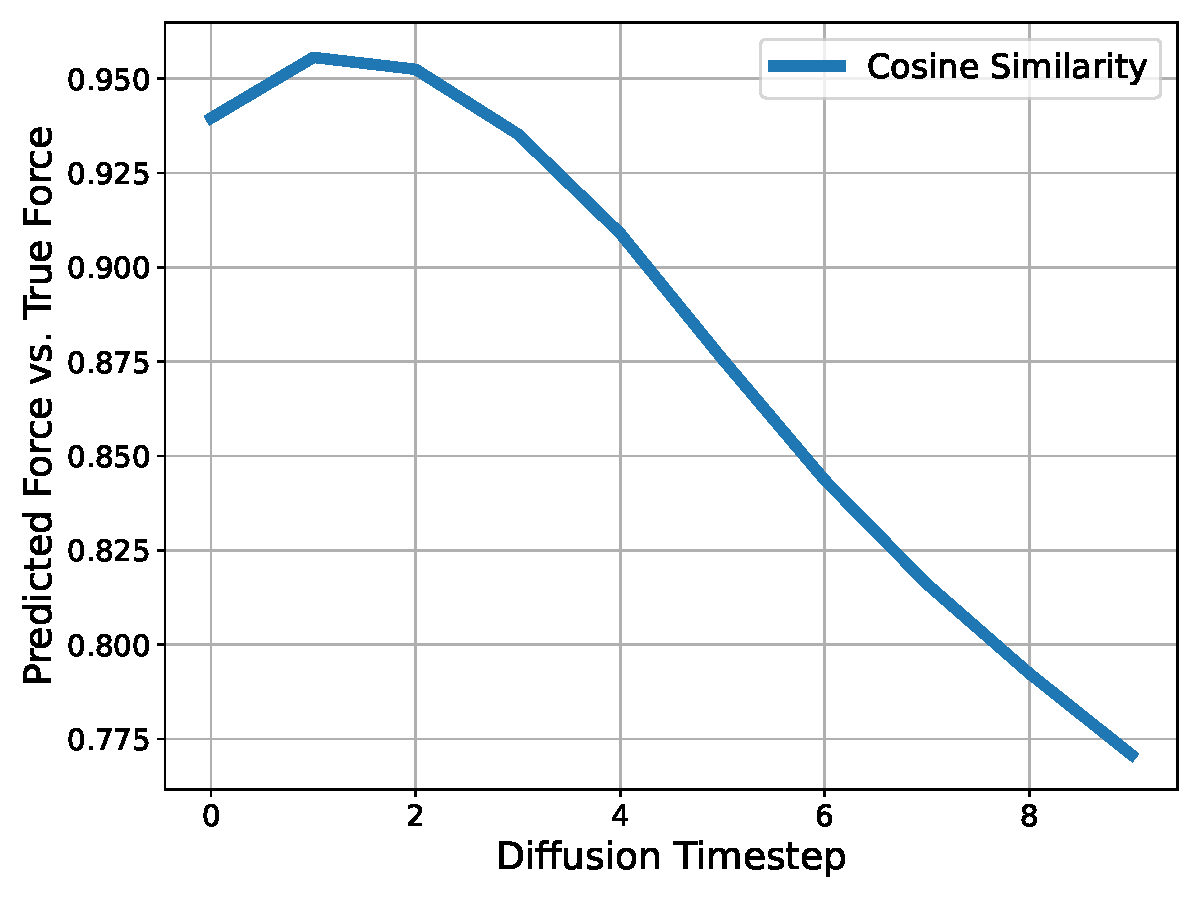
\includegraphics[width=\linewidth]{Figures/cosine_similarity_mb.pdf}
        \caption{\textbf{Müller-Brown.}}
        \label{fig:muller_brown}
    \end{subfigure}
    \hfill
    \begin{subfigure}[t]{0.49\linewidth}
        \centering
        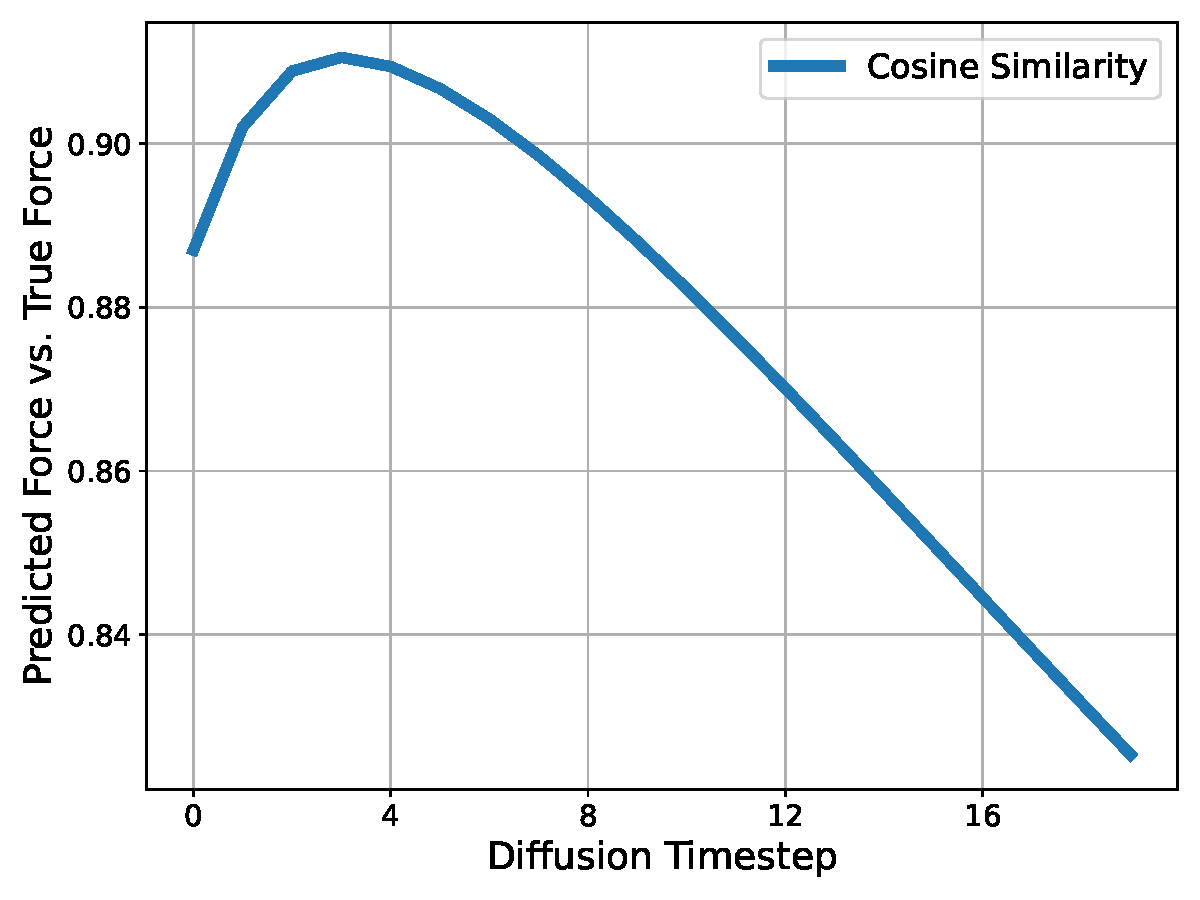
\includegraphics[width=\linewidth]{Figures/cosine_similarity_ala2.pdf}
        \caption{\textbf{Alanine Dipeptide.}}
        \label{fig:alanine_dipeptide}
    \end{subfigure}
    \vspace{2em}
    \caption{Cosine similarity between true force fields and learned force field from a DDPM's learned time-dependent score model $\mathbf{s}_\theta(\cdot, \tau_\text{opt})$ over different diffusion latent times $\tau_\text{opt}$. Results are averaged over all paths and atoms, for a Müller-Brown potential and Alanine Dipeptide. Notably, $\tau_\text{opt}=0$ is not the optimal time conditioning with respect to true force recovery for DDPM.}
    \label{fig:muller_alanine}
\end{figure*}


\section{Müller-Brown Potential Experiments}
\label{sec:mb_details}
We provide further details on the Müller-Brown experiments in Section \ref{sec:mb_results}. All experiments were performed on a single NVIDIA RTX A6000 GPU. 

\paragraph{Potential Parameters.} The exact form of the potential used is the following:

%A = [-1.73, -0.87, -1.47, 0.13] * 10
% a = 48, 32, 24, 16
% alpha = [-0.39, -0.39, -2.54, 0.273] * 1e-2
% beta = [0, 0, 4.30, 0.23] * 1e-2
% gamma = [-3.91, -3.91, -2.54, 0.273] * 1e-2
% b = [8, 16, 32, 24]

\begin{align*}
    U(x,y) &= -17.3 e^{-0.0039(x-48)^2 - 0.0391(y-8)^2} \\
    &\quad -8.7 e^{-0.0039(x-32)^2 - 0.0391(y-16)^2} \\
           &\quad - 14.7 e^{-0.0254(x -24)^2 + 0.043 (x-24)(y-32) -0.0254 (y-32)^2} \\
           &\quad + 1.3 e^{0.00273 (x-16)^2 + 0.0023 (x-16)(y-24) + 0.00273 (y-24)^2}
\end{align*}


% Doobs params
% \begin{align*}
%     U(x,y) &= -200 e^{-(x-1)^2 - 10y^2} - 100 e^{-x^2 - 10(y-0.5)^2} \\
%            &\quad - 170 e^{-6.5(x + 0.5)^2 + 11 (x+0.5)(y-1.5) - 6.5 (y-1.5)^2} \\
%            &\quad - 15 e^{0.7(x+1)^2 + 0.6 (x+1)(y-1) + 0.7 (y-1)^2}
% \end{align*}

This generates the potential shown in \fref{fig:mb_result}. \fref{fig:mb_analytical} shows OM optimization using the analytical potential as the force field. Increasing the diffusivity yields paths that cross higher energy barriers, aligning with physical intuition. The results with the diffusion model in Section \ref{sec:mb_results} align with the paths derived from the analytical potential, confirming the validity of the diffusion model as an approximation of the forces.   

\begin{figure}
    \centering
    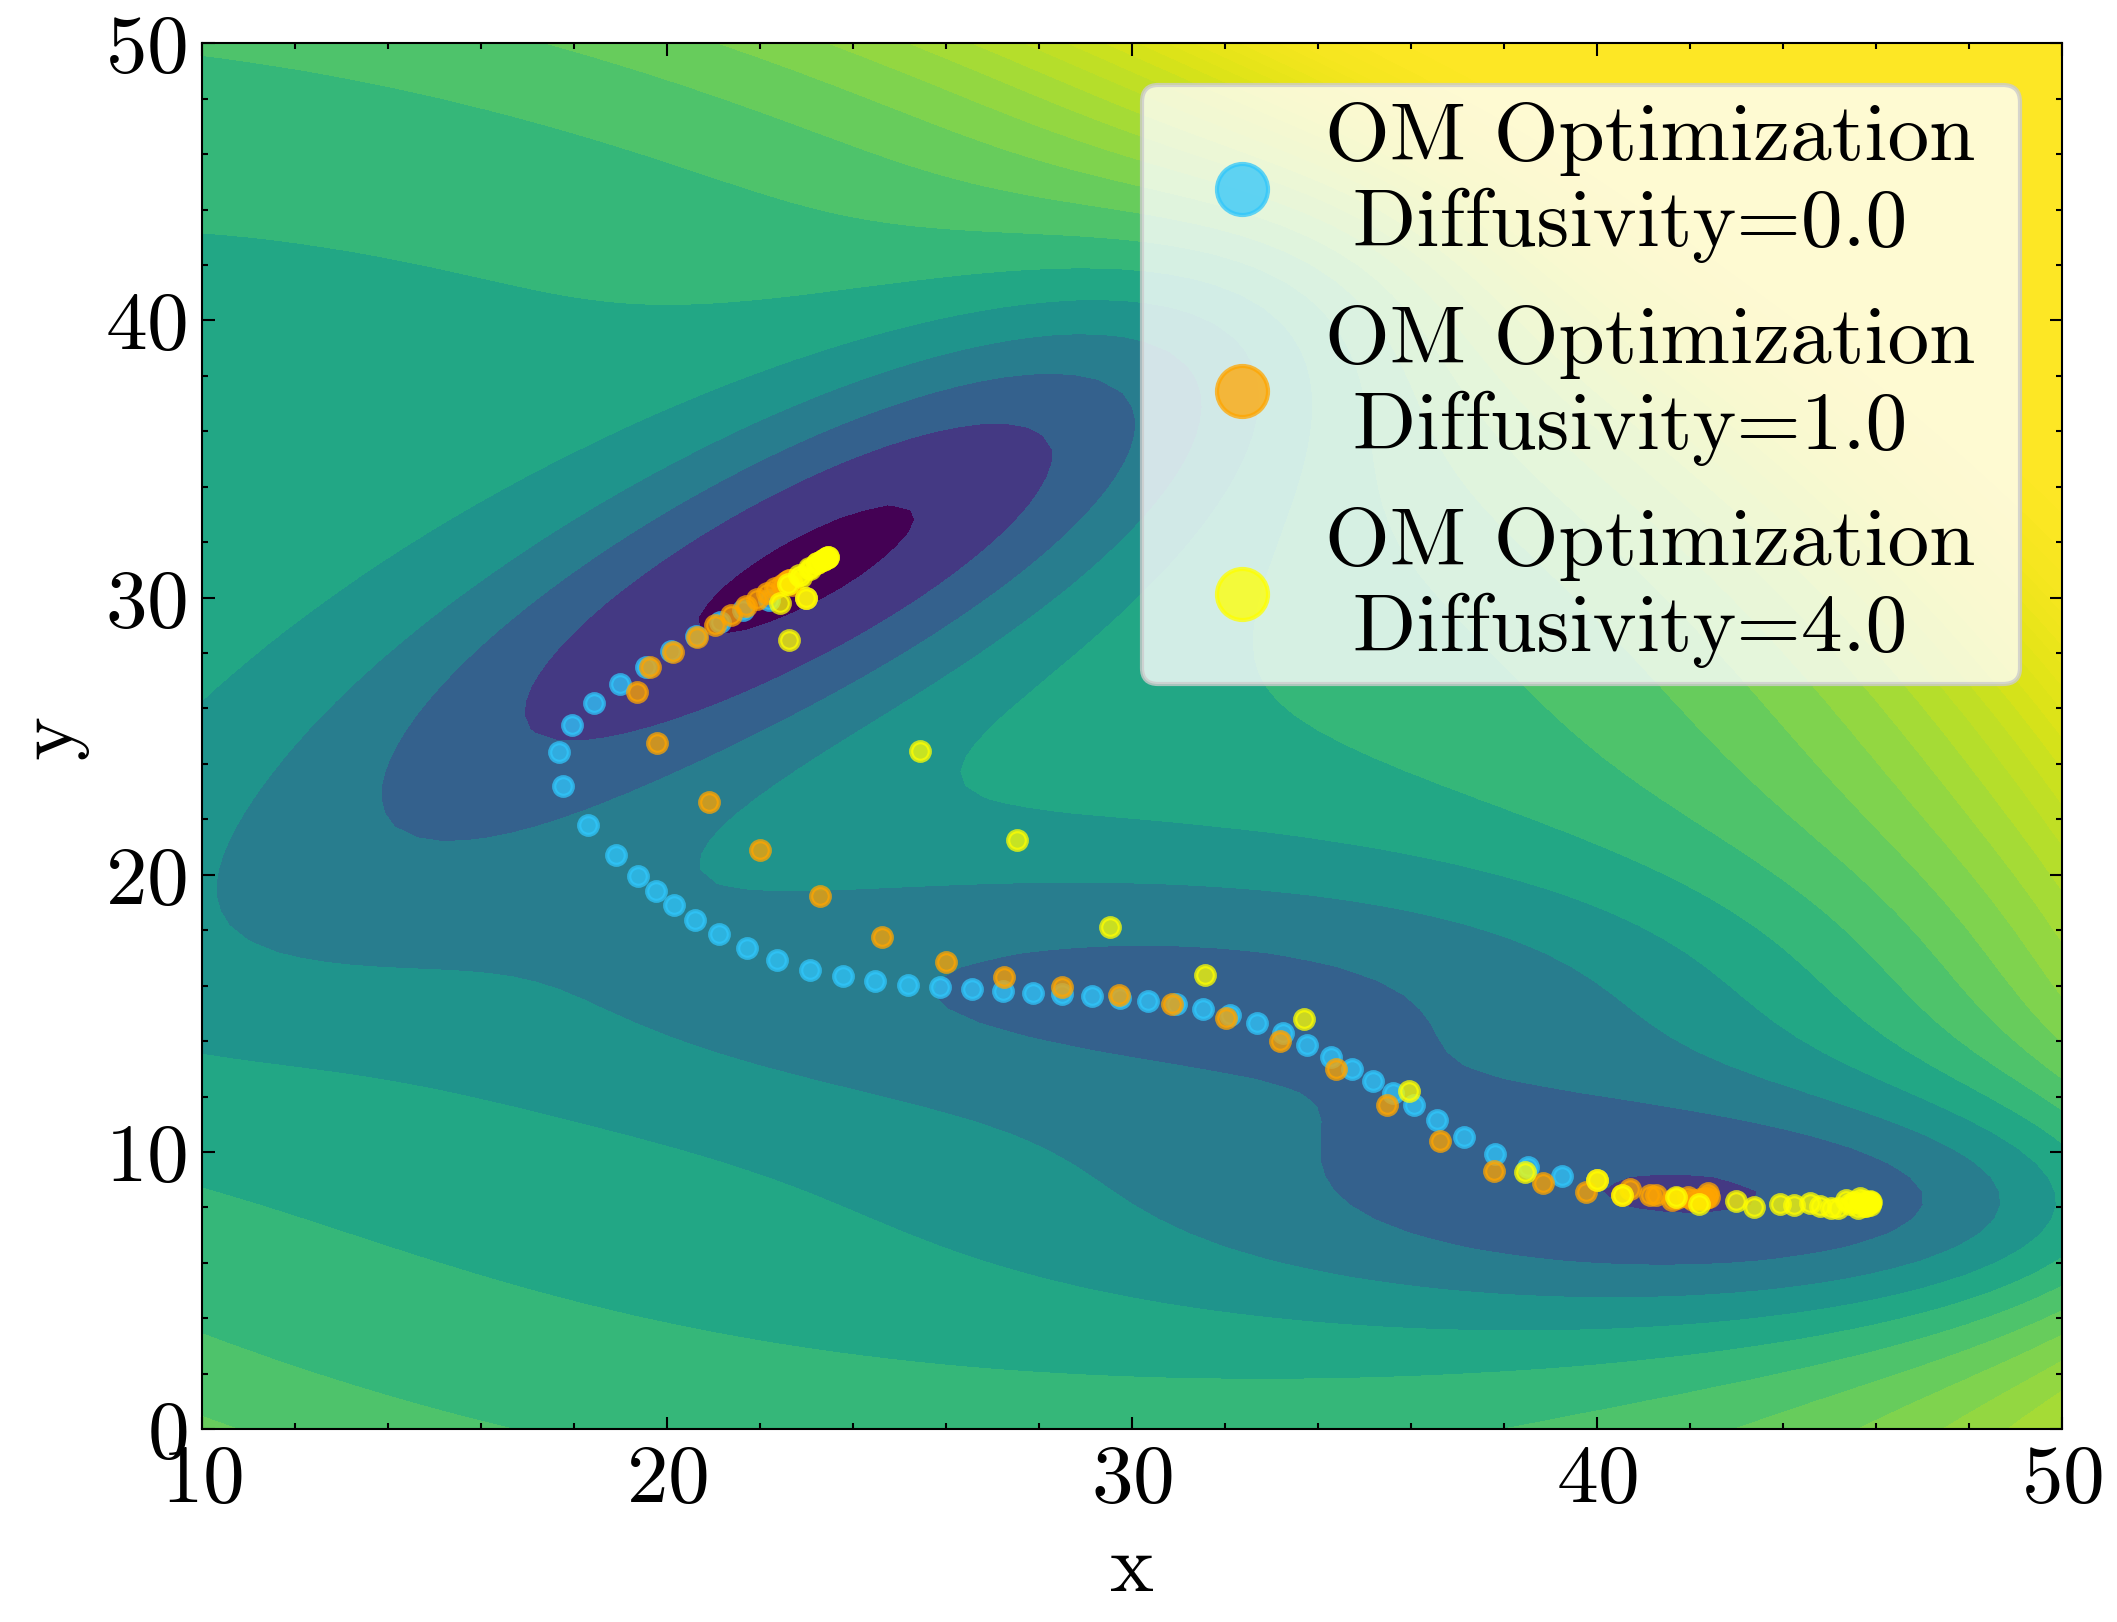
\includegraphics[width=0.5\linewidth]{Figures/mb_analytical_om.png}
    \caption{\textbf{OM optimization can be done with an analytical potential.} We show paths generated with OM optimization using the analytical potential with a timestep of 1, a friction of 1, and multiple diffusivities. Higher diffusivities, corresponding to higher temperatures in physical interpretation, can cross higher energy barriers, aligning with physical intuition.}
    \label{fig:mb_analytical}
\end{figure}

\paragraph{Data generation.} To ensure that the transition region is adequately represented with relatively short simulation times, we choose initial conditions for the simulations by uniformly sampling the transition path resulting from OM optimization under the true MB potential. We generate training data by running unbiased, constant-temperature simulations with the MB potential under Langevin dynamics. We run 1,000 parallel simulations for 1,000 steps, yielding a total of 1 million datapoints. Of these, 800,000 are used for training, and 200,000 are reserved for validation.

\paragraph{Training.} We then train a standard denoising diffusion model on this dataset, with the denoising model parameterized by a 3-layer MLP with a GELU activation \citep{hendrycks2023gaussianerrorlinearunits} and a hidden dimension of 256. The model is trained for 10 epochs, with a batch size of 4096 and a learning rate of $1\text{e}-3$ using the Adam optimizer \citep{kingma2017adammethodstochasticoptimization}. 

\begin{figure}
    \centering
    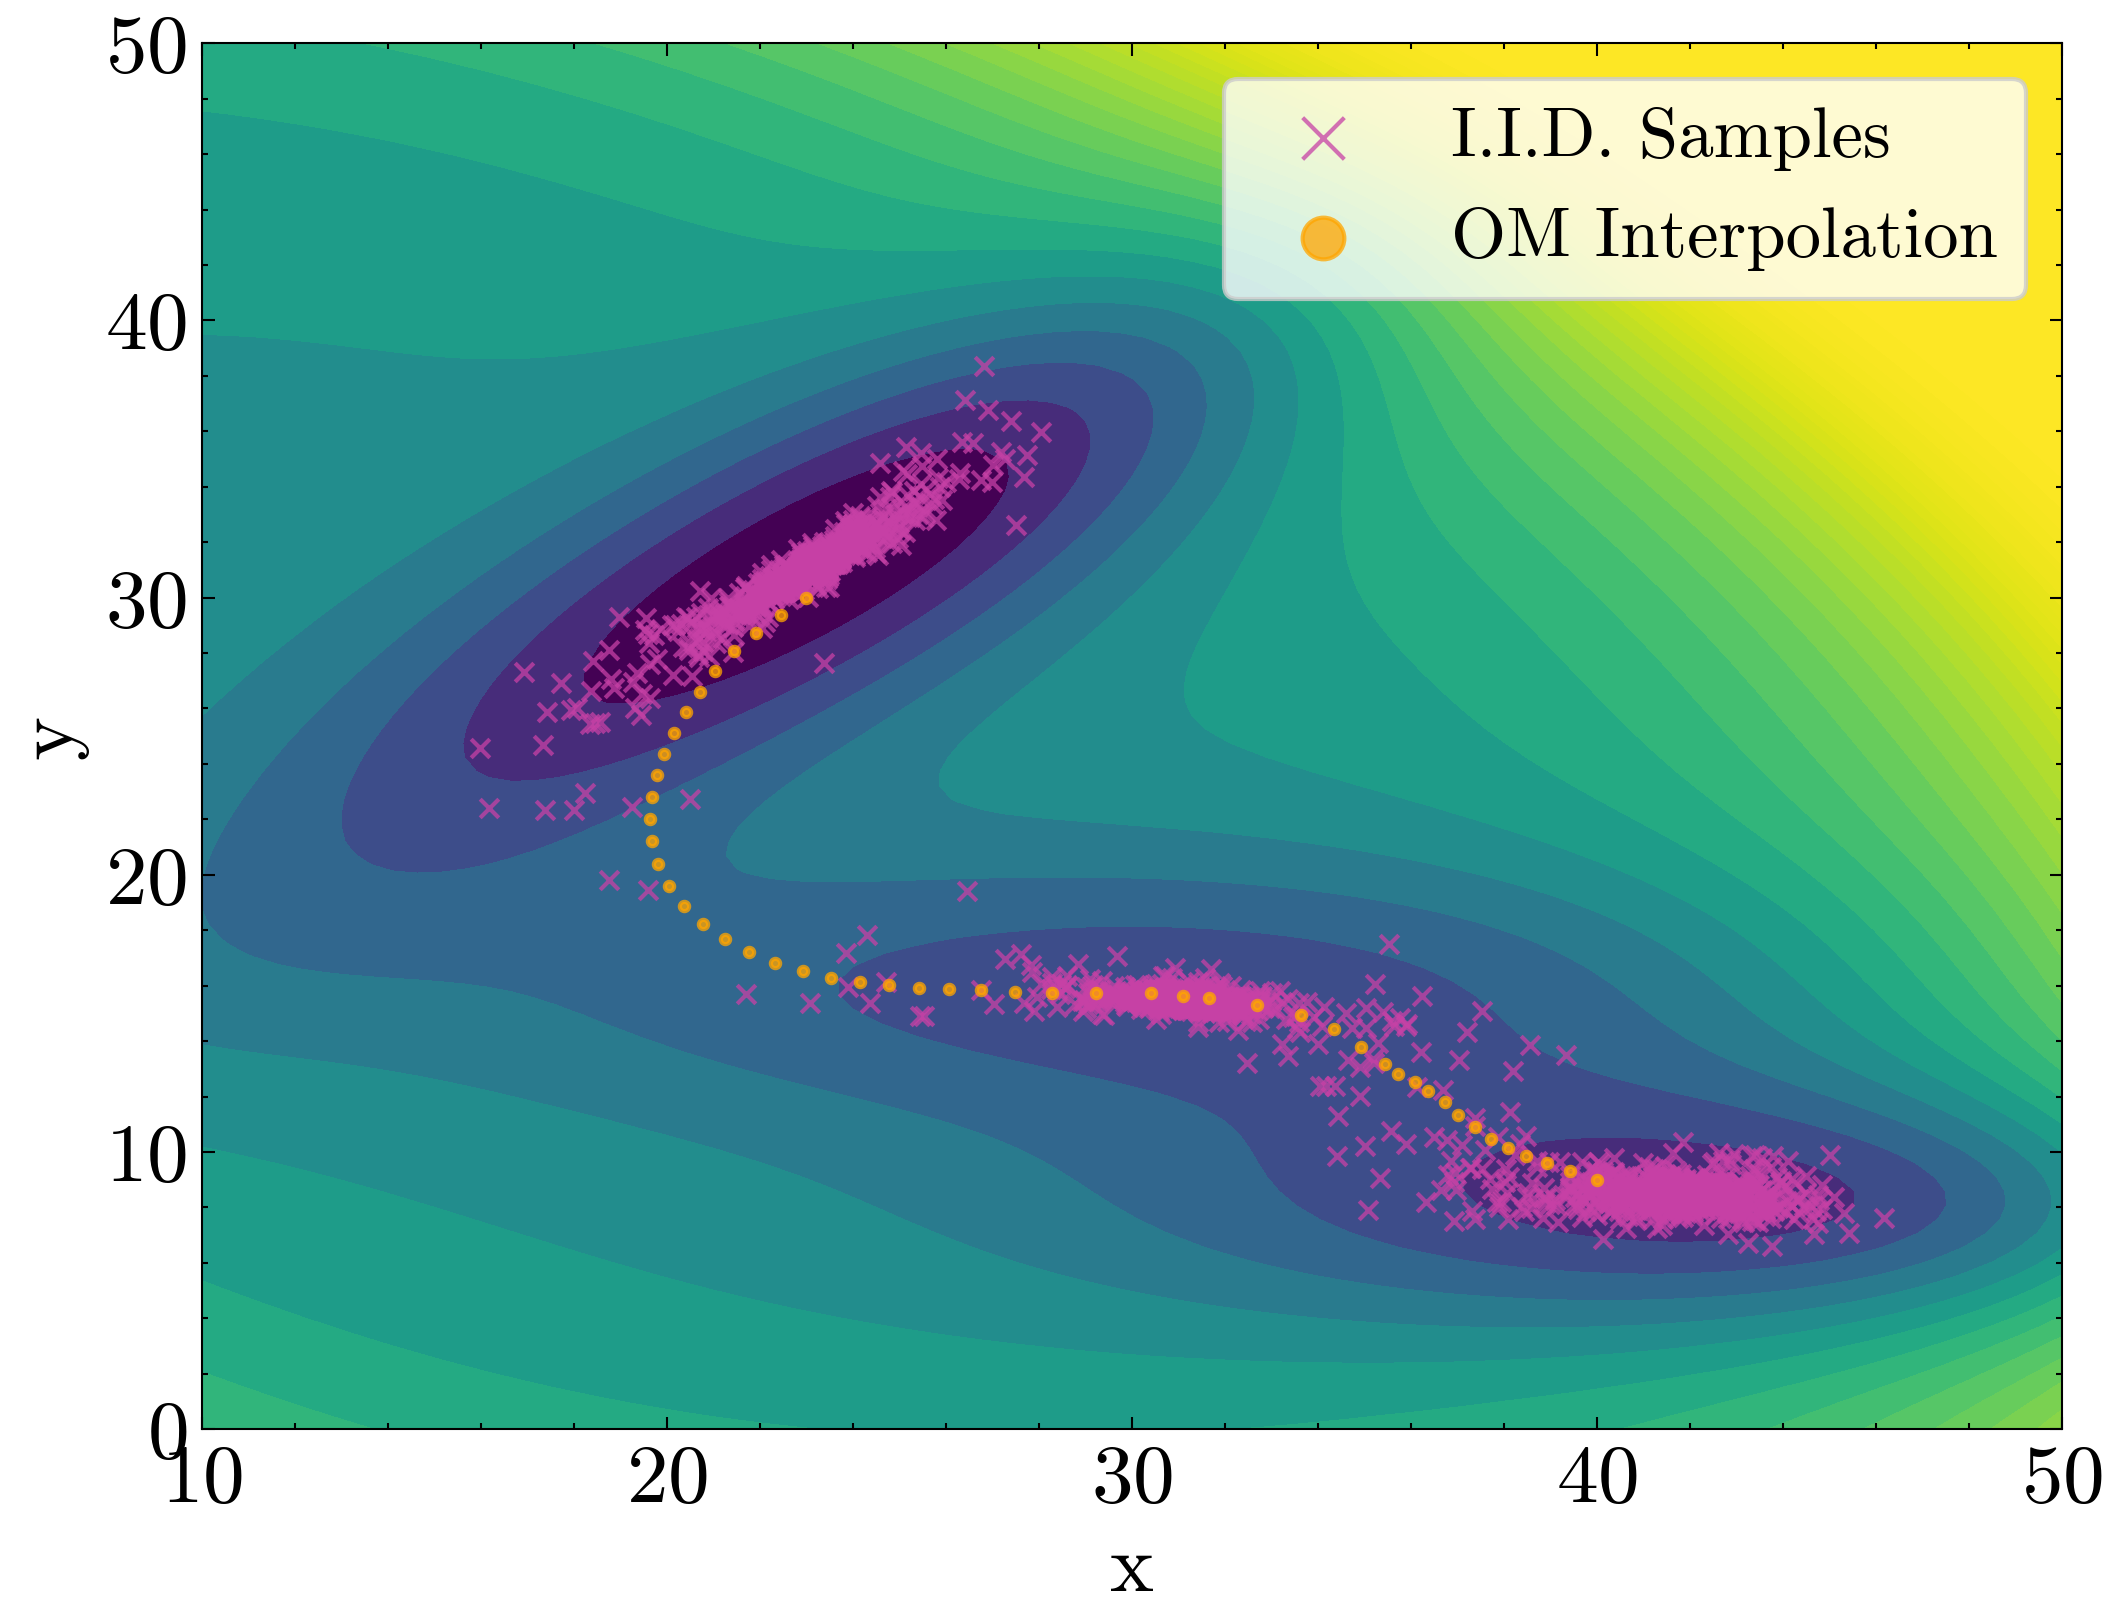
\includegraphics[width=0.5\linewidth]{Figures/mb_flowmatch.png}
    \caption{\textbf{OM optimization from a flow matching model}. The analogous experiment to \fref{fig:mb_analytical}, but using a flow matching model trained on Müller-Brown data, and using the extracted score via \eqref{eq:flow_force} for OM optimization. Since the stochastic encoding/decoding processes of flow matching models are deterministic and the Müller-Brown setting has a single minimal landscape, the encoding/decoding scheme in itself cannot generate diversity in this setting. The trajectory is generated at diffusivity $D=0$.}
    \label{fig:mb_flowmatching}
\end{figure}

% \sr{TODO: michael consolidate this figure with the old one}
% \begin{figure*}[h]
%     \centering
%     \includegraphics[width=1.0\linewidth]{Figures/rebuttal_flowmatch_interp.png}
%     \caption{OM-optimized trajectory (red line) with respect to a flow matching model trained on M\"uller-Brown data, plotted over $1\mathrm{e}6$ i.i.d. samples from the same flow matching model.}
%     \label{fig:flowmatch_new}
% \end{figure*}

% \paragraph{Correspondence Between Learned Vector Fields and True Forces.}

% We examine the similarity of the learned vector fields of the diffusion and flow matching models to the true forces, which are analytically computable for 2D Müller-Brown. The generative models are accurate estimates of the true forces (see Figure \ref{fig:mb_cos_sim}).

% \begin{figure}
%     \centering
%     \includegraphics[width=0.75\linewidth]{Figures/cos_sim.png}
%     \caption{\textbf{Diffusion model has high cosine similarity to true forces.}}
%     \label{fig:mb_cos_sim}
% \end{figure}


\paragraph{Energy Laplacian Term.} We estimate the Laplacian of the potential energy surface by using the Hutchinson Trace Estimator (see Section \ref{sec:om_details}). As shown in \fref{fig:hutch}, one random vector ($N=1$) is enough to capture the local minima and the energy barrier using the Hutchinson Trace Estimator, so we use $N=1$ in our experiments. Using more random vectors gives a less noisy estimate of the Laplacian, trading off accuracy for computational expense. 


\begin{figure}[h]
    \centering
    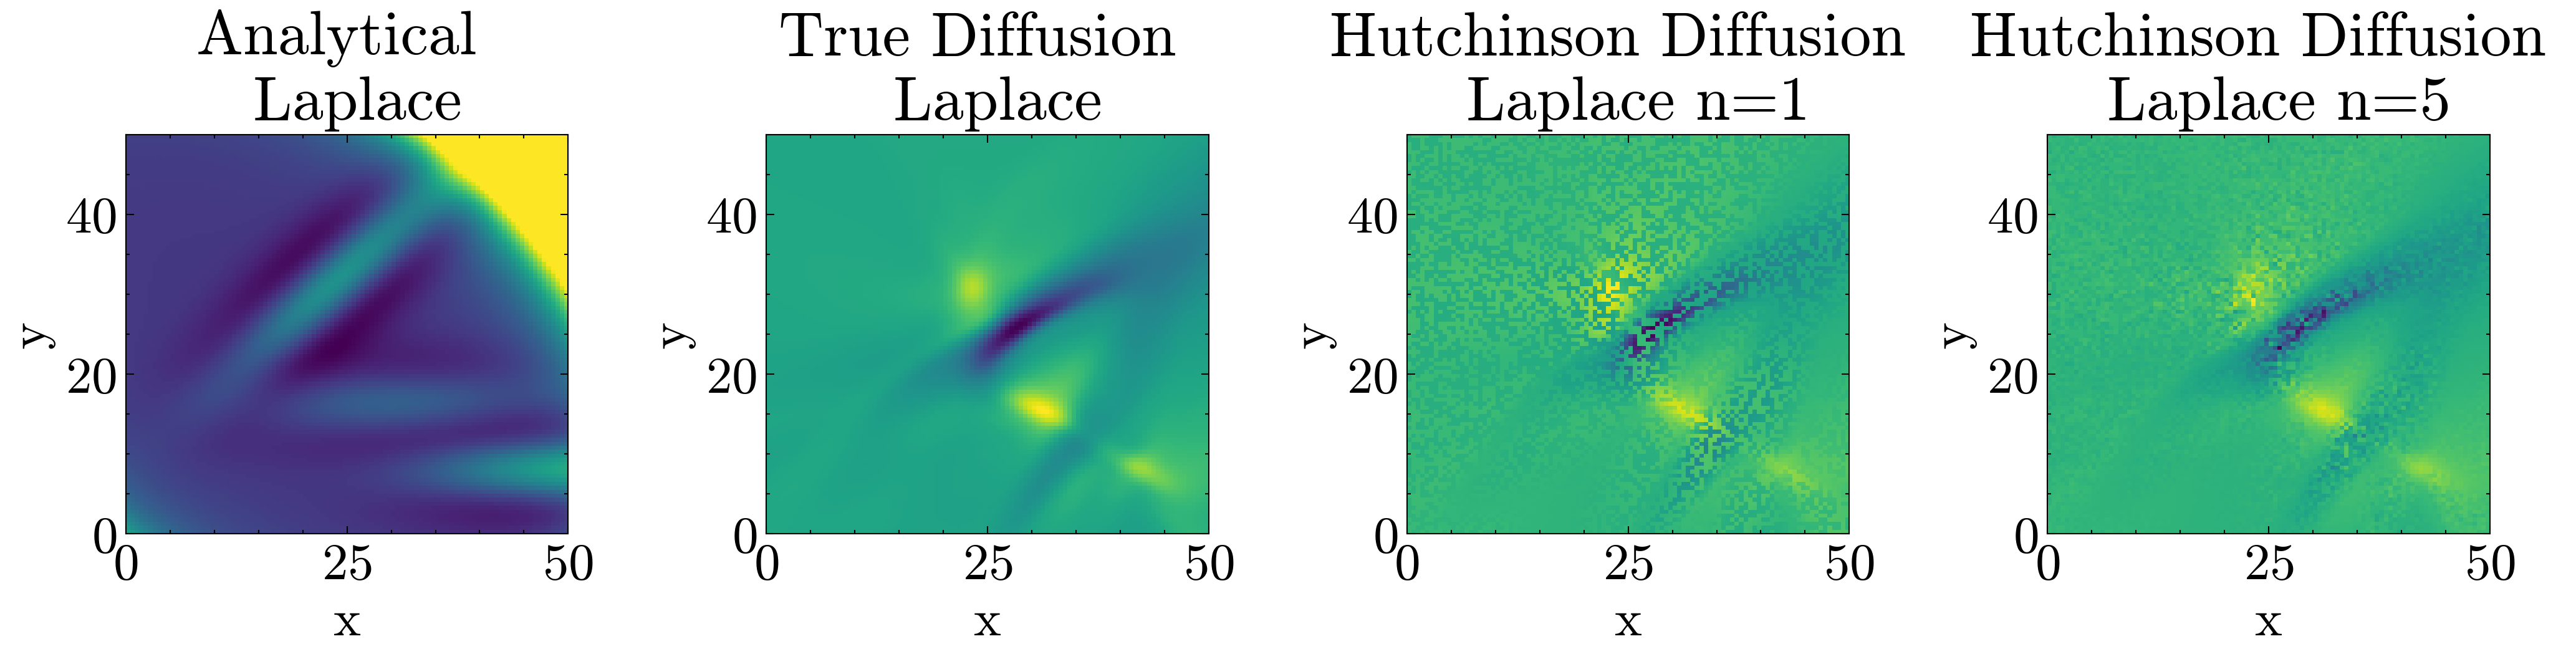
\includegraphics[width=0.95\linewidth]{Figures/laplacians_w_hutch_old_params.png}
    \caption{\textbf{Hutchinson Trace Estimator accurately estimates the Laplacian.} The diffusion model learns an estimate of the Laplacian that captures the Müller-Brown energy wells. The Hutchinson Trace Estimator efficiently approximates this Laplacian, and the estimate becomes less noisy when using more random samples.} 
    \label{fig:hutch}
\end{figure}

\paragraph{OM Optimization Details.} We pick two points on the potential energy surface (PES) at alternate ends of the transition barrier as target points for interpolation. The hyperparameters for the OM optimization are given in Table \ref{tab:om_optimization_details_mb}

%The initial guess for the interpolation is given by a linear interpolation in the latent space of the diffusion model

\begin{table}[h]
\caption{Hyperparameters used for OM action optimization on the Müller-Brown potential with diffusion.}
\label{tab:om_optimization_details_mb}
\scriptsize
\centering
\begin{tabular}{lc} % Retaining the original tabular layout
    \toprule
    \textbf{Hyperparameter} & \textbf{Value}\\
    \midrule
    Number of Generated Paths & 50\\
        Action Type & Full\\
        Initial Guess Time ($\tau_\text{initial}$) & 8\\
        Optimization Time ($\tau_\text{opt}$) & 8\\
        Optimization Steps & 200\\
        Optimizer & Adam \\
        Learning Rate & 0.2 \\
        Path Length ($L$) & 50\\
        Action Timestep ($\Delta t$) & 0.01\\
        Action Friction ($\gamma$) & 0.01\\
        Action Diffusivity ($D$) & 0, 1.0, 4.0\\
    \bottomrule
\end{tabular}
\end{table}

\paragraph{Committor Function and Rate Estimation}
We provide additional details on the committor function and transition rate estimation experiment presented in Section \ref{sec:mb_results}. 

According to transition path theory \cite{vanden2006towards}, for a transition event between endpoints $\mathcal{A}, \mathcal{B} \in \Omega$, the committor function $q(\xx)$, captures the probability that a trajectory initiated at $\xx_0 = \xx$ reaches $\mathcal{B}$ before $\mathcal{A}$:

\begin{equation}
\label{eq:committor_full}
q(\xx) = \mathbb{E}[h_\mathcal{B}(\xx_\tau) \mid \xx_0 = \xx]; \quad
\tau = \argmin_{\substack{t \in [0, +\infty)}} \quad  \left \{ \xx_t \in \mathcal{A} \cup \mathcal{B} :
\xx_0 = \xx \right \},
\end{equation}
where $h_\mathcal{B}$ is the indicator function for reaching state $\mathcal{B}$. The transition state ensemble is formally defined as the level set $\{ \xx \in \Omega: q(\xx) = 0.5 \}$. The committor function $q(\xx)$ can be used to estimate transition rates between a reactant state $\mathcal{A}$ and product state $\mathcal{B}$ using the following formula \cite{vanden2006towards}:
\begin{equation}
    \label{eq:committor_rate_equiv}
    k = \frac{k_BT}{\gamma}\int_{\xx \in \Omega} p(\xx) |\nabla_\xx q(\xx)|^2 dx = \frac{k_BT}{\gamma}\langle |\nabla_\xx q(\xx)|^2 \rangle_\Omega,
\end{equation}
where $p(\xx)$ is the probability density under the Boltzmann distribution and $\Omega$ is the configuration space. Thus, with a differentiable estimate of the committor function, we can compute reaction rates as an ensemble average over samples from $p(\xx)$. By applying the Backward Kolmogorov Equation (BKE) and Vainberg’s Theorem, we can show that the committor function is the solution to the following functional optimization problem \cite{hasyim2022supervised}:

\begin{equation}
    \label{eq:func_opt}
    q(\xx) = \argmin_{\widetilde{q}} \mathcal{L}[\widetilde{q}] =  \argmin_{\widetilde{q}}\frac{1}{2} \langle |\nabla_\xx \widetilde{q}(\xx)|^2 \rangle_{\Omega \backslash \mathcal{A} \cup \mathcal{B}},
\end{equation}
subject to the boundary conditions $\widetilde{q}(\xx) = 0, \xx \in \partial \mathcal{A}; \widetilde{q}(\xx) = 1, x \in \partial \mathcal{B}$. Thus, we can train a neural network approximation to the committor function $q_\theta(\xx)$ by extremizing the following loss function:

\begin{equation}
    \label{eq:committor_loss}
    L(\theta) = \frac{1}{2} \langle | \nabla_\xx q_\theta(\xx)| ^2 \rangle_{\Omega \backslash \mathcal{A} \cup \mathcal{B}} + \lambda_\mathcal{A} \frac{1}{2} \langle q_\theta(\xx) ^2 \rangle_\mathcal{A} + \lambda_\mathcal{B} \frac{1}{2} \langle (1-q_\theta(\xx))^2 \rangle_\mathcal{B}
\end{equation}

The first term minimizes the BKE functional, and the second and third terms enforce the boundary conditions with penalty strengths $\lambda_\mathcal{A}$ and $\lambda_\mathcal{B}$, respectively. The ensemble averages in the loss, which are high-dimensional integrals whose computational cost grows exponentially with system size, are in practice replaced by importance-sampled Monte Carlo averages over a dataset of samples $\mathcal{D}_\text{train} = \{ x_i \}_{i=1}^N
$ from MD simulations, MCMC, or any enhanced sampling method (such as OM optimization). Once trained, the neural network committor function $q_\theta(\xx)$ can be used to estimate the rate via Eqn \ref{eq:committor_rate_equiv}, substituting $q_\theta(\xx)$ in place of $q(\xx)$, and averaging over $\mathcal{D}_\text{train}$ instead of the intractable full ensemble average over $\Omega$. 

\begin{equation}
    k_\theta = \frac{k_BT}{\gamma}\langle |\nabla_\xx q_\theta(\xx)|^2 \rangle_\Omega \approx \hat{\mathbb{E}}_{\xx \sim \mathcal{D}_\text{train}} |\nabla_\xx q_\theta(\xx)|^2 
\end{equation}

Notice that the neural network estimate of the rate $k_\theta$ is equivalent (up to constants) to the BKE functional loss $\mathcal{L}[\widetilde{q}]$. The primary challenge with learning the committor function in this way is the issue of sampling: the optimization problem is dominated by rare events with large values of $|\nabla_\xx q_\theta(\xx)|^2$ (i.e events in the transition region). Therefore, if the transition region(s) are insufficiently sampled, the training procedure will likely fail to converge, and the estimate rate $k_\theta$ will be inaccurate. Therefore, committor and rate estimation using this method reduces to a rare event sampling problem. Inspired by \citet{hasyim2022supervised}, our idea is to use the transition paths obtained from our OM optimization procedure (shown in \fref{fig:mb_rates}a) as samples over which to minimize \eqref{eq:committor_loss}. Specifically, for the Müller-Brown potential, we first sampled more points by initiating unbiased Langevin dynamics simulations along the OM-optimized paths (100 simulations, each 50 ps long, $k_BT = 1$), using the diffusion model's score function at $\tau=0$ as the force field (we could have also used the analytical forces from the Müller-Brown potential). This resulted in a collection of points $\mathcal{D}_\text{train} = \{ x_i \}_{i=1}^N
$ (shown in \fref{fig:mb_rates}b). To account for the biased initial conditions of the simulations, we reweight the samples in $\mathcal{D}_\text{train}$ to the underlying Boltzmann distribution using the reweighting factors 
\begin{equation}
    w_i = \frac{\frac{e^{-\beta U(x_i)}}{p_\text{OM}(x_i)}}{\Sigma_i \frac{e^{-\beta U(x_i)}}{p_\text{OM}(x_i)}},
\end{equation}
where $\beta = \frac{1}{k_BT}$, $U(\xx)$ is the analytical Müller-Brown potential energy, and $p_\text{OM}$ is the empirical density of $\mathcal{D}_\text{train}$, obtained via binning. We train a 5-layer MLP with a hidden dimension of 64 and a sigmoid activation function to approximate the committor function. The model is trained for 2000 steps with a batch size of 4096, using an Adam optimizer with a learning rate of 0.0001 and a cosine decay scheduler. The boundary condition loss weights are $\lambda_\mathcal{A} = \lambda_\mathcal{B} = 20$. The final estimated committor function profile is shown in \fref{fig:mb_rates}c. We obtain a transition rate estimate of $1.3 \times 10^{-5}$, compared with the true rate of $5.4 \times 10^{-5}$ obtained by solving the Backward Kolmogorov Equation numerically using a finite-element method in FEniCS \cite{baratta2023dolfinx}. 

\begin{figure*}[h]
    \centering
    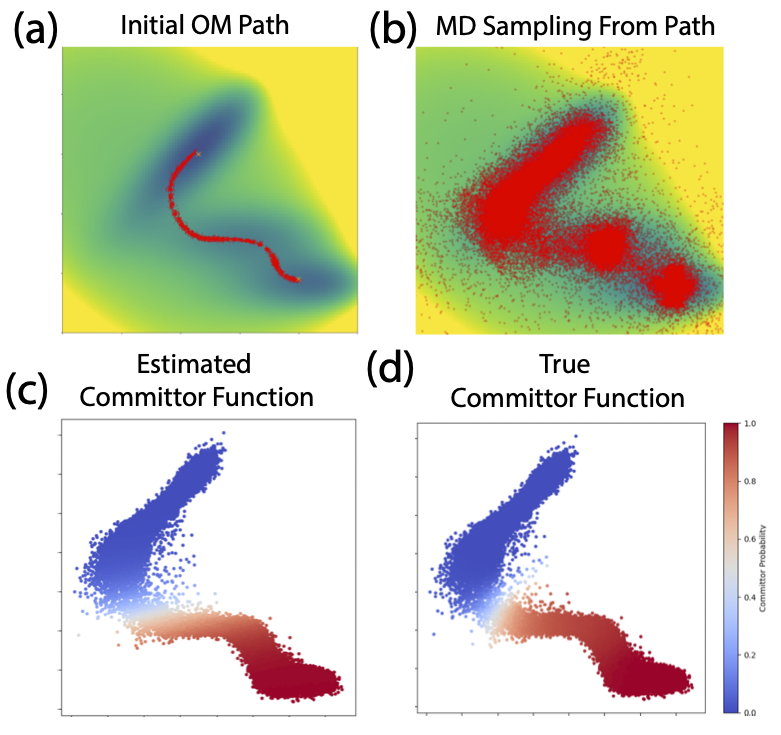
\includegraphics[width=0.7\linewidth]{Figures/mb_rates.png}
    \caption{\textbf{Efficient committor and transition rate estimation on the 2D Müller-Brown potential using OM optimization.} \textbf{(a)} Initial OM optimized transition path with a pretrained denoising diffusion model, using $\tau_\text{opt}=4$ and 100 paths. \textbf{(b)} Subsequent diversification of the sampled transition paths by performing unbiased Langevin dynamics simulations initiated along the OM optimized paths (100 simulations, each 10,000 steps, $k_BT = 1$) with the diffusion model's score function at $\tau=0$. \textbf{(c)} Predicted values of the committor function $q(\xx)$, obtained via minimizing $\langle |\nabla_\xx q_\theta(\xx)|^2 \rangle_\Omega$, where $\langle \cdot \rangle_\Omega$ denotes an ensemble average over the samples collected in part b) and the committor function $q_\theta(\xx)$ is parameterized by a 5 layer MLP  with hidden dimension of 64 and sigmoid activation. \textbf{(d)} True committor function calculated by solving the Backward Kolmogorov Equation numerically using a finite-element method in FEniCS. The reaction rate $k$ is computed via the relation $k = \frac{k_BT}{\gamma}\langle |\nabla_\xx q(\xx)|^2 \rangle_\Omega$. Our predicted reaction rate is $1.3 \times 10^-5$, compared with the true rate of $5.38 \times 10^-5$.
    }
    \label{fig:mb_rates}
\end{figure*}





%\paragraph{Impact of Conservative Vector Field Parameterization.}

%\tk{TODO}.

\section{Alanine Dipeptide Experiments.}
\label{sec:alanine_dipeptide_details}
We present additional results on the alanine dipeptide results in Section \ref{sec:alanine_dipeptide_results}.

\paragraph{Details on Traditional Enhanced Sampling Baselines.}
For MCMC, we report metrics found in \cite{du2024doob} for the fixed-length, two-way, exact method. We implement metadynamics ourselves with Ramachadran angles as CVs. We use a hill height of 0.2kcal/mol, a width of 10Å, and a temperature of 300K. We report the number of force field (or generative model score) evaluations required per 1,000 step transition path (a batched computation over many samples is considered to be one evaluation). 

% \begin{figure*}[h]
%     \centering
%     \includegraphics[width=1.0\linewidth]{Figures/hills.png}
%     \caption{\textbf{Potential of mean force obtained by metadynamics} The barrier is around 6-8kcal/mol.}
%     \label{fig:metadynamics}
% \end{figure*}

\paragraph{Diffusion Model Training.}
We construct a training dataset from MD simulations of alanine dipeptide at 1000K (a large temperature is chosen to promote the inclusion of transition regions in the data). We then train a diffusion model on these samples, using the Graph Transformer architecture described in \sref{sec:fastfolding_details}. We train models for 50,000 steps, using an Adam optimizer with a learning rate of 0.0004 and a cosine annealing schedule reducing to a minimum learning rate of 0.00001. We use an exponential moving average with $\alpha = 0.995$. The diffusion model uses 1,000 integration steps at inference time.


\paragraph{OM Optimization Details.}
We choose a path length of $L=300$ and noise/denoise by 300 steps (out of 1,000) to initialize via Algorithm \ref{alg:gen_initial_guess}, then conduct OM optimization for 50,000 steps, fixing latent diffusion time $\tau_\text{opt}=3$. $\gamma$ and $\Delta t$ are set to 0.7 and 1e-4 respectively. After OM optimization, we run a short energy minimization procedure for 1400 steps using the Amber \textit{ff19SB} classical force-field to relax structures, followed by OM optimization using BFGS algorithm that required around 21,000 steps.

\paragraph{Calculating Free Energy Barriers with Umbrella Sampling.}
Since we optimized with the truncated OM action \eqref{eq:final_OM_truncated} we obtained minimum energy paths. To compute free energy barriers that are necessary for reaction rate predictions and comparisons with literature, we employ some sampling to estimate the entropic contribution. On alanine dipeptide, we use the following procedure to obtain free energy profiles along the OM-optimized paths.
\begin{enumerate}
\item Perform umbrella sampling \cite{torrie1977nonphysical}: short, 10ps, simulations with a harmonic string potential centered around the points that define the original minimum energy path. The spring constant used had value of 5 $\text{kcal}/\text{mol}/\text{rad}^2$
\item Fit a collective variable (CV) on the resulting samples. We choose Principal Component Analysis (PCA).
\item Employ the WHAM algorithm \cite{kumar1992weighted} to obtain the reweighted potential of mean force, shown in \fref{fig:free_energy}b.
\end{enumerate}

\section{Fast-Folding Protein Experiments}
\label{sec:fastfolding_details}

We present additional details on the fast-folding protein results in Section \ref{sec:fastfolders}. All experiments were performed on a single NVIDIA RTX A6000 GPU. 

\paragraph{MD Simulations with Diffusion Model}
To assess the computational efficiency and accuracy of our OM optimization relative to alternative methods of sampling the configurational space (see \fref{fig:fastfolders}a and b), we run Langevin MD simulations for varying lengths of time (up to 12 ns) using the diffusion model's score function as an effective force field \cite{arts2023two}, with a timestep of 2 fs. To ensure a fair comparison, we set the number of parallel MD trajectories to be the same as the number of transition paths sampled with OM optimization. 

\paragraph{Markov State Model Construction.}
We provide further details on the Markov State Model analysis used to evaluate the quality of transition paths for the fast-folding protein experiments. We largely follow the procedure described in \citet{jing2024generative}.

We perform k-means clustering of the reference MD simulations into 20 clusters using the top 2 Time Independent Component (TIC) dimensions, which are fit on the pairwise distances and dihedral angles of the protein configurations. We then fit a Markov State Model (MSM) with a lagtime of 200ps (the frequency at which the simulations were saved) to obtain a transition probability matrix $T$ between the 20 discrete states in the MSM (e.g, $T_{j,k} = p (s_{t+1} = k | s_t = j)$, where $s_t$ and $s_{t+1}$ are the states at time $t$ and $t+1$). This constitutes the reference MSM.

To evaluate transition paths sampled from our OM optimization method, we first discretize them under the reference MSM (i.e represent them as a sequence of cluster indices between 1 and 20). We subsample the paths to be of length 20. From this, we compute the probability of the path under the reference MSM via:

We also sample 1,000 discrete, reference paths of length $L=20$ (corresponding to a transition time of $200 \text{ps} \times 20 = 4 \text{ns}$) from the reference MSM, conditioned on the start and end states $s_1$ and $s_{L}$ (these are the cluster indices of the transition endpoints $\xx^{(0)}$ and $\xx^{(L)}$) . This can be achieved by sampling states $s_2 \ldots s_{19}$ iteratively as 
\begin{equation}
    s_{t+1} \sim \frac{T_{:, s_{L}}^{(L-t-1)} T_{s_{L}, :}}{T_{s_t, s_{L}}^{(L-t)}},
\end{equation}
where the superscipt denotes a matrix exponential. See \citet{jing2024generative} for precise details. 

With both the reference and generated discretized paths, we compute the following metrics:
\begin{enumerate}
    \item \textbf{Jensen-Shannon Divergence.} Consider the probability of each MSM state based on the frequency at which it is visited in the discretized paths. We compute these probabilities for both the reference and generated paths, and compute the JSD between the resulting categorical distributions.
    \item \textbf{Transition Negative Log Likelihood.} The average negative log likelihood of a transition from one discretized MSM state to the next, averaged over transitions from all generated paths with nonzero probability under the reference MSM. Since there are $L-1$ individual transitions for a path of length $L$, under the Markovian assumption the average negative log likelihood of a transition is given by $-\frac{1}{L-1}\log P(s_1 \ldots s_L) = -\frac{1}{L-1}\sum_{t=1}^{L-1} \log \Bigg( \frac{T^{(L-t-1)}_{s_t, s_L} \cdot T_{s_t, s_{t+1}}}{T^{(L-t)}_{s_t, s_L}} \Bigg)$.
    \item \textbf{Fraction of Valid Paths.} The fraction of generated paths with nonzero probability under the reference MSM.
\end{enumerate}


When considering replicate MD simulations of different lengths (e.g 1 $\mu$s, 10 $\mu$s), we fit a MSM to the simulations using the same discretized clusters as were used to fit the reference MSM, and sample 1,000 paths of length $L=20$ in the same way described above. 

We note that the reported metrics are sensitive to the choice of the MSM trajectory length $L$ used for the reference simulations. Varying $L$ changes the time horizon of the transition and yields qualitatively different reference paths. Since we chose $L=20$, the reported metrics reflect the correspondence of generated paths with true paths of length 4 ns. We also find that in practice, the optimal choice of $\Delta t$ in the OM action (i.e., the choice that yields the best MSM metrics as defined above) results in time horizons $T_p = L \Delta t$ (where $L$ here is the number of path discretization points during OM optimization) considerably smaller than the reference time horizon of $4$ ns (e.g., for the typical choices of $L = 200$, $\Delta t= 1 fs$, we have $T_p = 0.2 ps$). In other words, OM optimization yields accelerated transition dynamics, because it largely bypasses local/minor fluctuations that would occur in an actual MD simulation. 

\paragraph{Committor Function Analysis.} 
The committor function $q(\xx)$ (see \sref{sec:mb_results} for definition) is obtainable as the solution to the steady-state backward Kolmogorov equation (BKE) \cite{hasyim2022supervised}, which is generally infeasible to solve directly or numerically for high-dimensional systems. For the fast-folding proteins, we obtain an empirical estimate of the committor function by dividing the TIC configuration space of each protein into $100^2$ discrete bins, and replacing the expectation in \eqref{eq:committor_full} with an empirical average over trajectories starting from each bin in the reference MD simulations from \citet{lindorff2011fast}. The resulting committor estimates for the fast-folding proteins are shown in \fref{fig:protein_committors}.

\begin{figure*}[h]
    \centering
\includegraphics[width=\linewidth]          {Figures/protein_committors.jpg}
    \caption{\textbf{Empirical committor landscapes for fast-folding proteins.} The committor is computed by binning the conformational space into $100^2$ bins and measuring the frequency at which reference MD trajectories initiated in each bin reach the target state before the start state. The empirical transition ensemble (shown in black) is defined as the level set $\left \{ \xx : 0.45 \leq q(\xx) \leq 0.55 \right \}$.}
    \label{fig:protein_committors}
\end{figure*}


\paragraph{Model Architecture and Training.} Our denoising diffusion and flow matching generative models are parameterized by a Graph Transformer architecture identical to what was used in \citet{arts2023two} (in the case of diffusion, we use the exact pretrained model from \citet{arts2023two}). To summarize, nodes are featurized by the ordering of each residue in the overall sequence, while edges are featurized by the pairwise $C_\alpha$-$C_\alpha$ distances. Nodes and edges are then jointly treated as tokens for input to the Transformer, which updates the token representations. A scalar output is obtained by summing learned linear projections of the token representations. Both the denoising diffusion vector field $\epsilon_\theta$ and the flow model velocity field $v_\theta$ are parameterized as the gradient of the final scalar output of the model with respect to the input $C_\alpha$ coordinates.

For denoising diffusion, we use the pretrained models from \citet{arts2023two}. For flow matching, we train our own models. We train models with 3 attention layers for 1 million iterations, using an Adam optimizer with a learning rate of 0.0004 and a cosine annealing schedule reducing to a minimum learning rate of 0.00001. We use an exponential moving average with $\alpha = 0.995$. The diffusion models use 1,000 integration steps at inference time, while the flow matching models use 10 steps. 

Protein-specific training and architecture hyperparameters are given in Table \ref{tab:fastfolder_architecture_training}.



\begin{table*}[h]
\caption{Architecture and training hyperparameters for diffusion and flow matching generative models on fast-folding proteins.}
\label{tab:fastfolder_architecture_training}
\scriptsize
\centering
    \begin{tabular}{lccccc}
        \toprule
        \textbf{Hyperparameter} & \textbf{Chignolin} & \textbf{Trp-cage} & \textbf{BBA} & \textbf{Villin} & \textbf{Protein G} \\
        \midrule
        Batch size & 512 & 512 & 512 & 512 & 256 \\
        Number of hidden features & 64 & 128 & 96 & 128 & 128 \\
        \bottomrule
    \end{tabular}
\end{table*}

\paragraph{OM Optimization Details.}

We list all the optimization hyperparameters used to perform OM optimization on the fast-folding proteins, for both diffusion and flow matching models, in Tables \ref{tab:om_optimization_details_diffusion} and \ref{tab:om_optimization_details_flow}.

\begin{table}[h]
\caption{Hyperparameters used for OM action optimization on fast-folding proteins with diffusion models.}
\label{tab:om_optimization_details_diffusion}
\scriptsize
\centering
\begin{tabular}{lccccc} % Retaining the original tabular layout
    \toprule
    \textbf{Hyperparameter} & \textbf{Chignolin} & \textbf{Trp-cage} & \textbf{BBA} & \textbf{Villin} & \textbf{Protein G} \\
    \midrule
    Number of Generated Paths & 8 & 8 & 32 & 4 & 4 \\
        Action Type & Truncated & Truncated & Full & Truncated & Truncated \\
        Initial Guess Time ($\tau_\text{initial}$) & 250 & 250 & 250 & 250 & 250 \\
        Optimization Time ($\tau_\text{opt}$) & 20 & 15 & 20 & 10 & 10 \\
        Optimization Steps & 5000 & 5000 & 5000 & 5000 & 5000 \\
        Optimizer & Adam & Adam & SGD & SGD & SGD \\
        Learning Rate & 0.2 & 0.2 & 1e-5 & 1e-5 & 1e-5 \\
        Path Length ($L$) & 200 & 200 & 200 & 200 & 200 \\
        Action Timestep ($\Delta t$) & 0.001 & 0.001 & 0.001 & 0.005 & 0.002 \\
        Action Friction ($\gamma$) & 1 & 1 & 1 & 1 & 1 \\
        Action Diffusivity ($D$) & 0 & 0 & 1 & 0 & 0 \\
    \bottomrule
\end{tabular}
\end{table}

\begin{table*}[h]
\caption{Hyperparameters used for OM action optimization on fast-folding proteins with flow matching models.}
\label{tab:om_optimization_details_flow}
\scriptsize
\centering
    \begin{tabular}{lccccc}
        \toprule
        \textbf{Hyperparameter} & \textbf{Chignolin} & \textbf{Trp-cage} & \textbf{BBA} & \textbf{Villin} & \textbf{Protein G} \\
        \midrule
        Number of Generated Paths & 8 & 8 & 32 & 4 & 4 \\
        Action Type & Truncated & Truncated & Full & Truncated & Truncated \\
        Initial Guess Time ($\tau_\text{initial}$) & 7 & 7 & 7 & 7 & 7 \\
        Optimization Time ($\tau_\text{opt}$) & 0.5 & 0.5 & 0.5 & 0.5 & 0.5 \\
        Optimization Steps & 5000 & 5000 & 5000 & 5000 & 5000 \\
        Optimizer & Adam & Adam & SGD & SGD & SGD \\
        Learning Rate & 0.2 & 0.2 & 1e-4 & 1e-4 & 1e-4 \\
        Path Length ($L$) & 200 & 200 & 200 & 200 & 200 \\
        Action Timestep ($\Delta t$) & 0.0008 & 0.0005 & 0.001 & 0.001 & 0.001 \\
        Action Friction ($\gamma$) & 1 & 1 & 1 & 1 & 1 \\
        Action Diffusivity ($D$) & 0 & 0 & 1 & 0 & 0 \\
        \bottomrule
    \end{tabular}
\end{table*}

% \paragraph{Complete Quantitative Results.} In Table \ref{tab:protein_sampling}, we report Markov State Model metrics for all fast-folding proteins, showing results of OM optimization with diffusion and flow matching, and Langevin MD simulations of varying lengths, using the diffusion model's score function as the force field.
% \begin{table*}[h]
% \centering
% \caption{Complete Markov State Model metrics for for fast-folding proteins. Metrics evaluated are: Fraction of Valid Paths (\textbf{FVP}), Transition Negative Log Likelihood Mean (\textbf{TNLLM}), and Jensen-Shannon Divergence (\textbf{JSD})}
% \label{tab:protein_sampling}
% \scriptsize
% \begin{tabular}{l l c c c}
% \toprule
% \textbf{Protein} & \textbf{Sampling Method} & \textbf{FVP (↑)} & \textbf{TNLLM (↓)} & \textbf{JSD (↓)} \\
% \midrule

% \multirow{3}{*}{Chignolin} 
% & Reference MD (1 $\mu$s) & 0 & N/A & 1\\
% & Reference MD (10 $\mu$s) & 1 & 1.73 & 0.035\\
% & Reference MD (50 $\mu$s) & 1 & 1.72  & 0.026\\
% & Reference MD (100 $\mu$s) & 1 &  1.71 & 0.016\\
% & OM Optimization (Diffusion) (ours) &  & & \\
% & OM Optimization (Flow Matching) (ours) & & & \\

% \midrule

% \multirow{3}{*}{Trp Cage} 
% & Reference MD (1 $\mu$s) &  &  & \\
% & Reference MD (10 $\mu$s) &  &  & \\
% & Reference MD (50 $\mu$s) & &  & \\
% & Reference MD (100 $\mu$s) & &  & \\
% & OM Optimization (Diffusion) (ours) &  & & \\
% & OM Optimization (Flow Matching) (ours) & & & \\


% \midrule

% \multirow{3}{*}{BBA} 
% & Reference MD (1 $\mu$s) &  &  & \\
% & Reference MD (10 $\mu$s) &  &  & \\
% & Reference MD (50 $\mu$s) & &  & \\
% & Reference MD (100 $\mu$s) & &  & \\
% & OM Optimization (Diffusion) (ours) &  & & \\
% & OM Optimization (Flow Matching) (ours) & & & \\

% \midrule

% \multirow{3}{*}{Villin} 
% & Reference MD (1 $\mu$s) &  &  & \\
% & Reference MD (10 $\mu$s) &  &  & \\
% & Reference MD (50 $\mu$s) & &  & \\
% & Reference MD (100 $\mu$s) & &  & \\
% & OM Optimization (Diffusion) (ours) &  & & \\
% & OM Optimization (Flow Matching) (ours) & & & \\

% \midrule

% \multirow{3}{*}{Protein G} 
% & Reference MD (1 $\mu$s) &  &  & \\
% & Reference MD (10 $\mu$s) &  &  & \\
% & Reference MD (50 $\mu$s) & &  & \\
% & Reference MD (100 $\mu$s) & &  & \\
% & OM Optimization (Diffusion) (ours) &  & & \\
% & OM Optimization (Flow Matching) (ours) & & & \\

% \bottomrule
% \end{tabular}
% \vspace{-10pt}
% \end{table*}

\paragraph{Comparison to Transition Paths from Reference MD Simulations.}

We directly compare our generated paths against the unbiased MD transition trajectories from the D.E.Shaw reference simulations \cite{lindorff2011fast}, finding that our paths sample the correct regions of phase space (\fref{fig:unbiased_md_tic}).

\begin{figure*}[h]
    \centering
    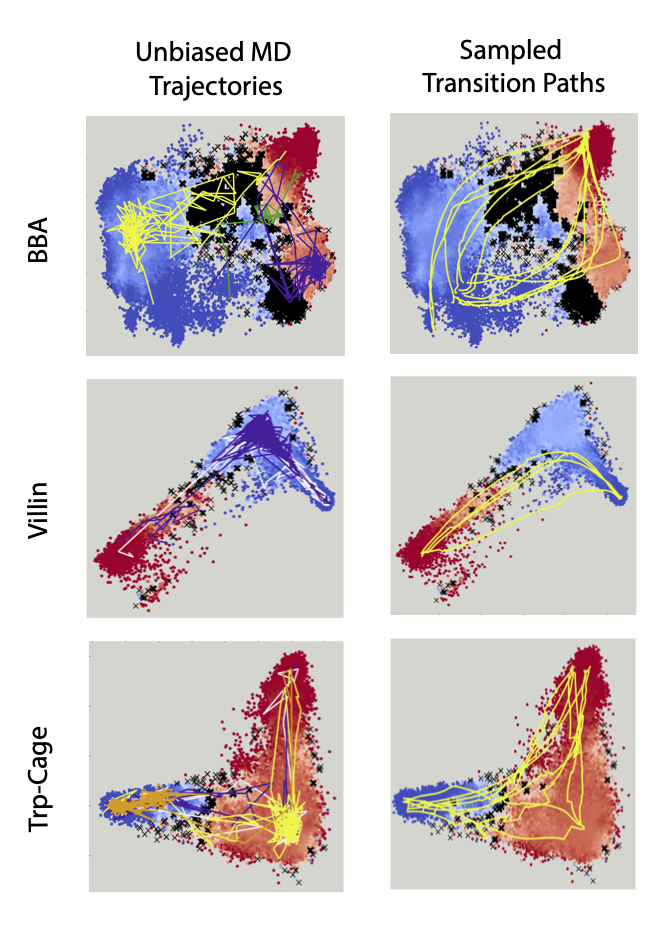
\includegraphics[width=0.5\linewidth]{Figures/unbiased_md_tic.png}
    \caption{Sample trajectories from reference, unbiased fast-folding protein MD simulations from D.E.Shaw (left) and paths sampled via OM optimization (right) overlaid on TICA plots with committor values shaded from blue to red. We observe strong agreement in the TICA space, with our OM paths traversing the same transition regions and exhibiting similar structural transitions. While the OM paths are smoother/do not contain the same fluctuations found in unbiased MD trajectories, they capture the same essential features. OM optimization somewhat oversamples transition paths which avoid energy wells. This could be improved by increasing the time horizon of the transition to accommodate time spent in kinetic traps.}
    \label{fig:unbiased_md_tic}
\end{figure*}

\paragraph{Visualization of Transition Paths.} In Figures \ref{fig:diffusion_tps_atoms}, \ref{fig:flow_tps_atoms}, and \ref{fig:more_tic_paths}, we provide additional visualizations of transition paths sampled by our diffusion and flow matching models for the fast folding proteins, both in TIC and atomic space.

\begin{figure*}[h]
    \centering
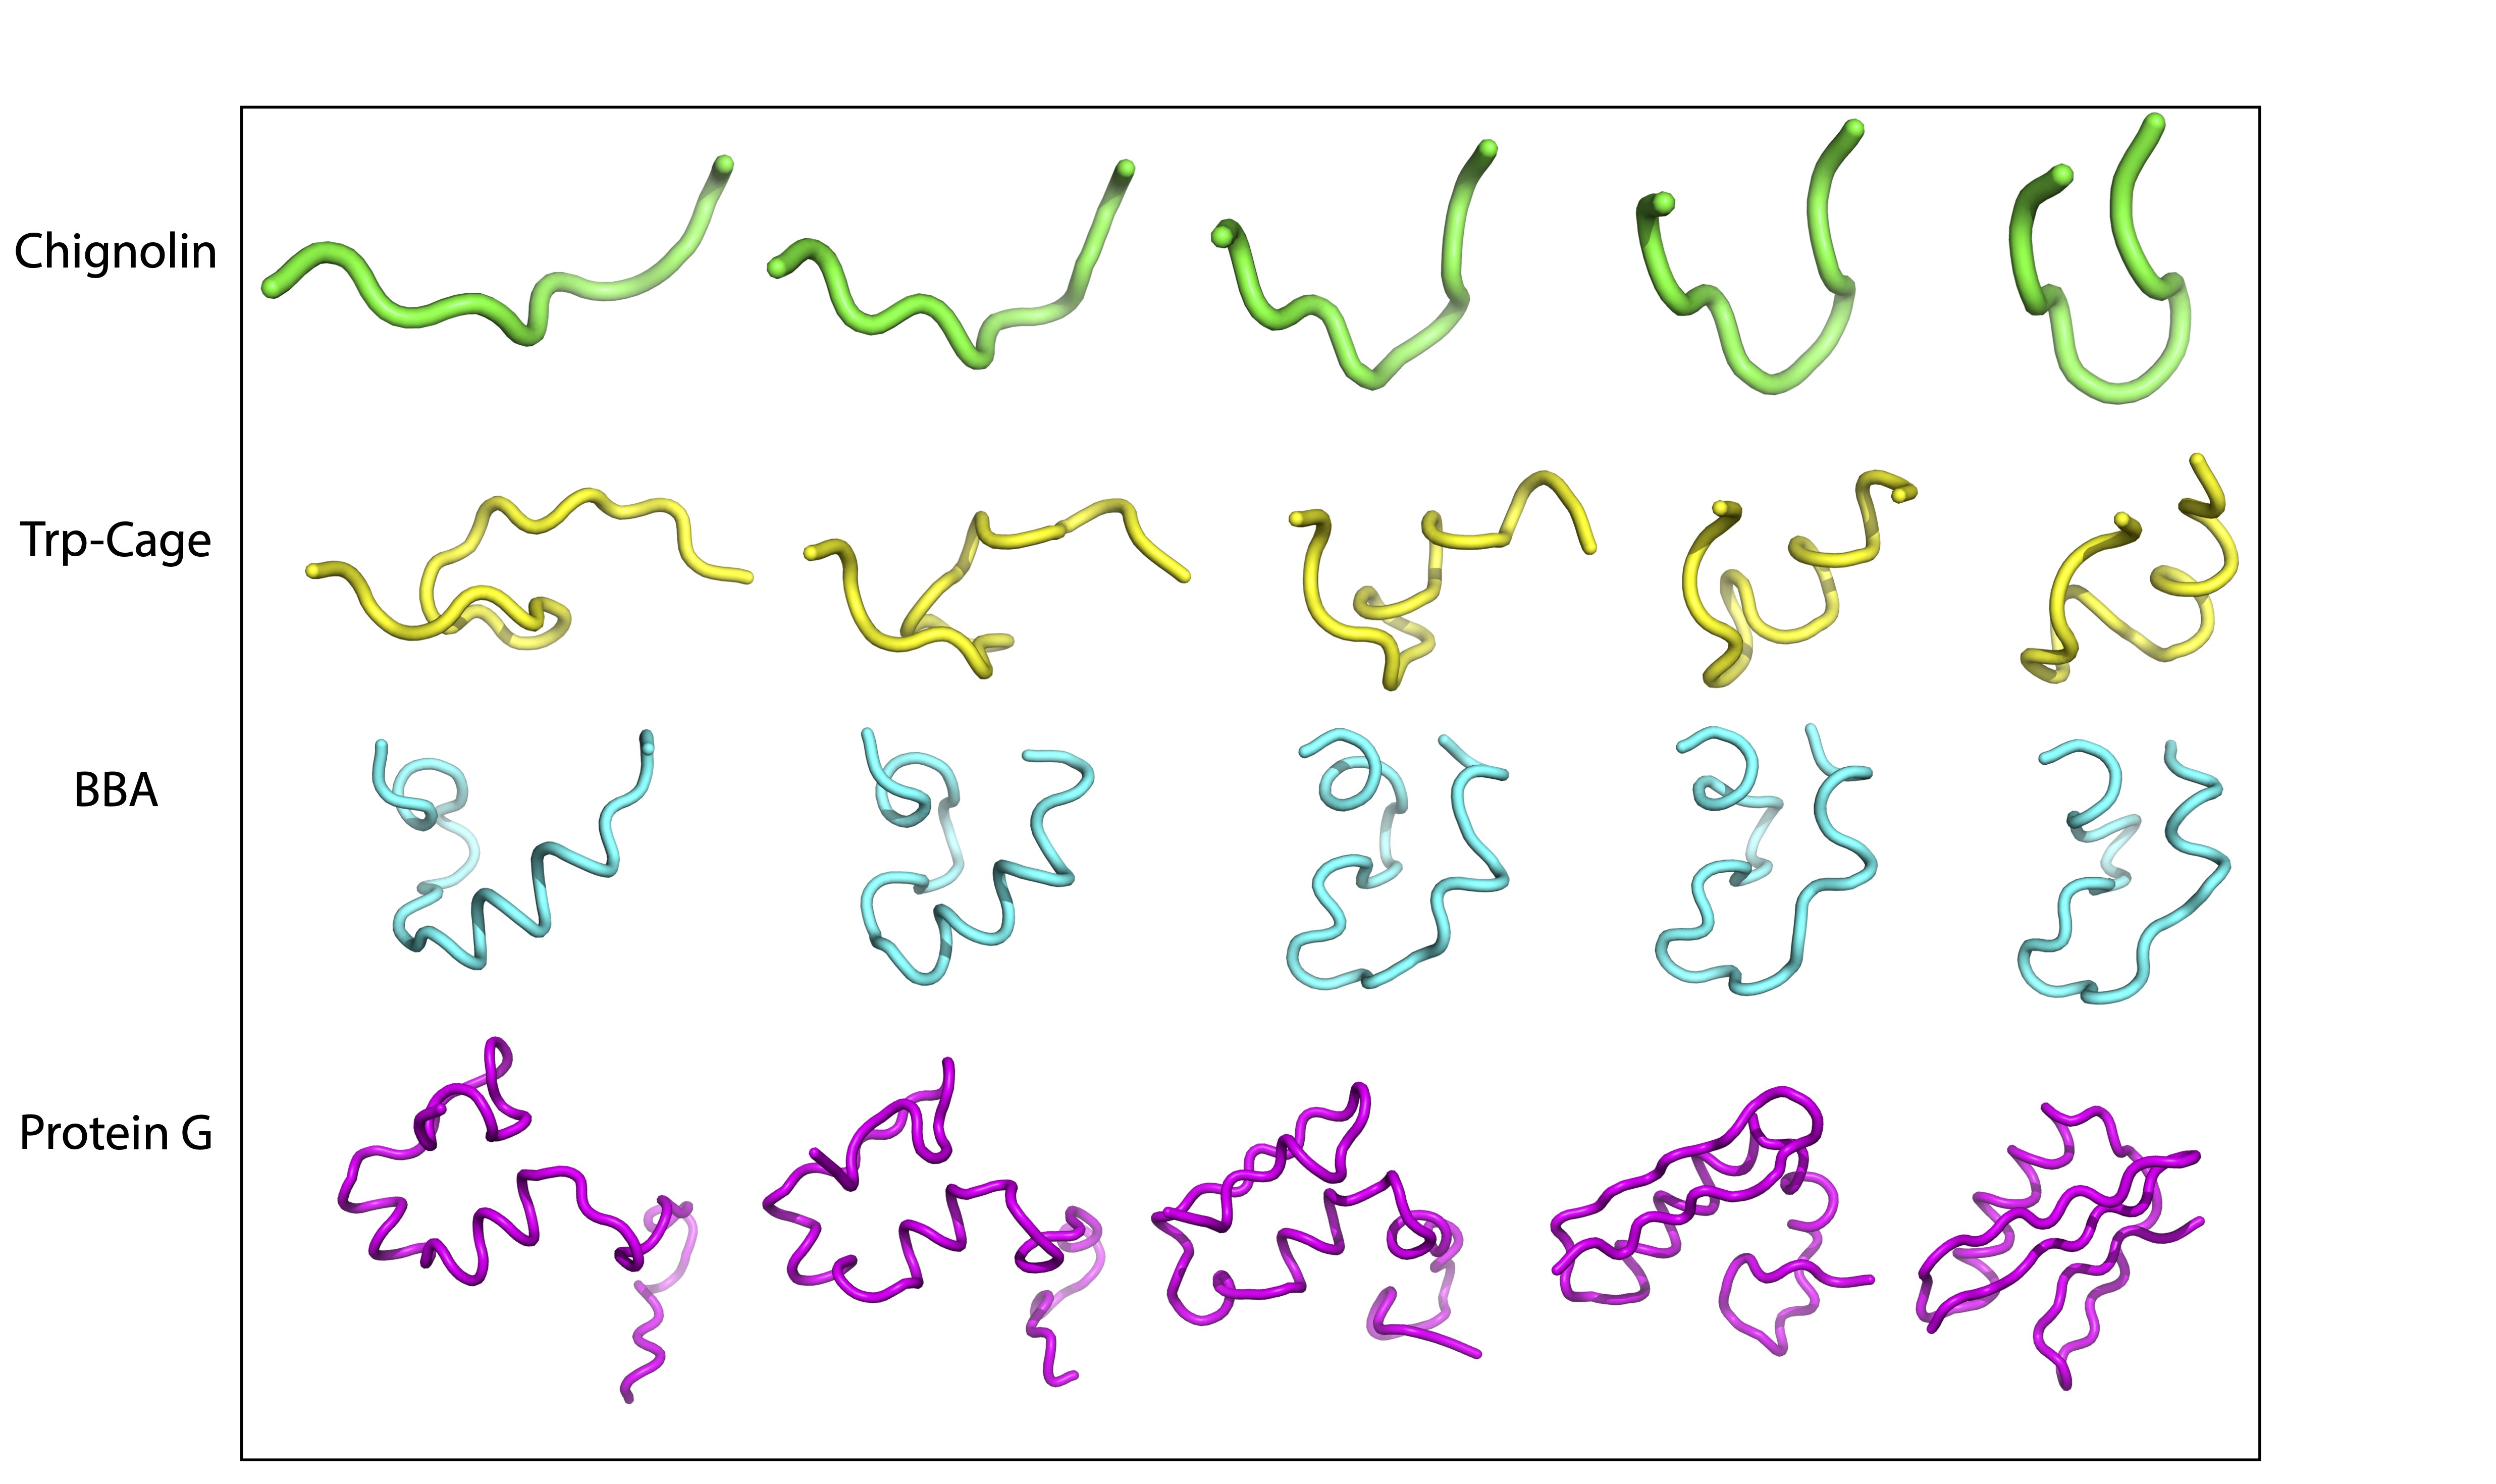
\includegraphics[width=\linewidth]          {Figures/diffusion_tps_atoms.png}
    \caption{Visualization of sampled transition paths from OM optimization with pretrained diffusion models for fast-folding proteins.}
    \label{fig:diffusion_tps_atoms}
\end{figure*}

\begin{figure*}[h]
    \centering
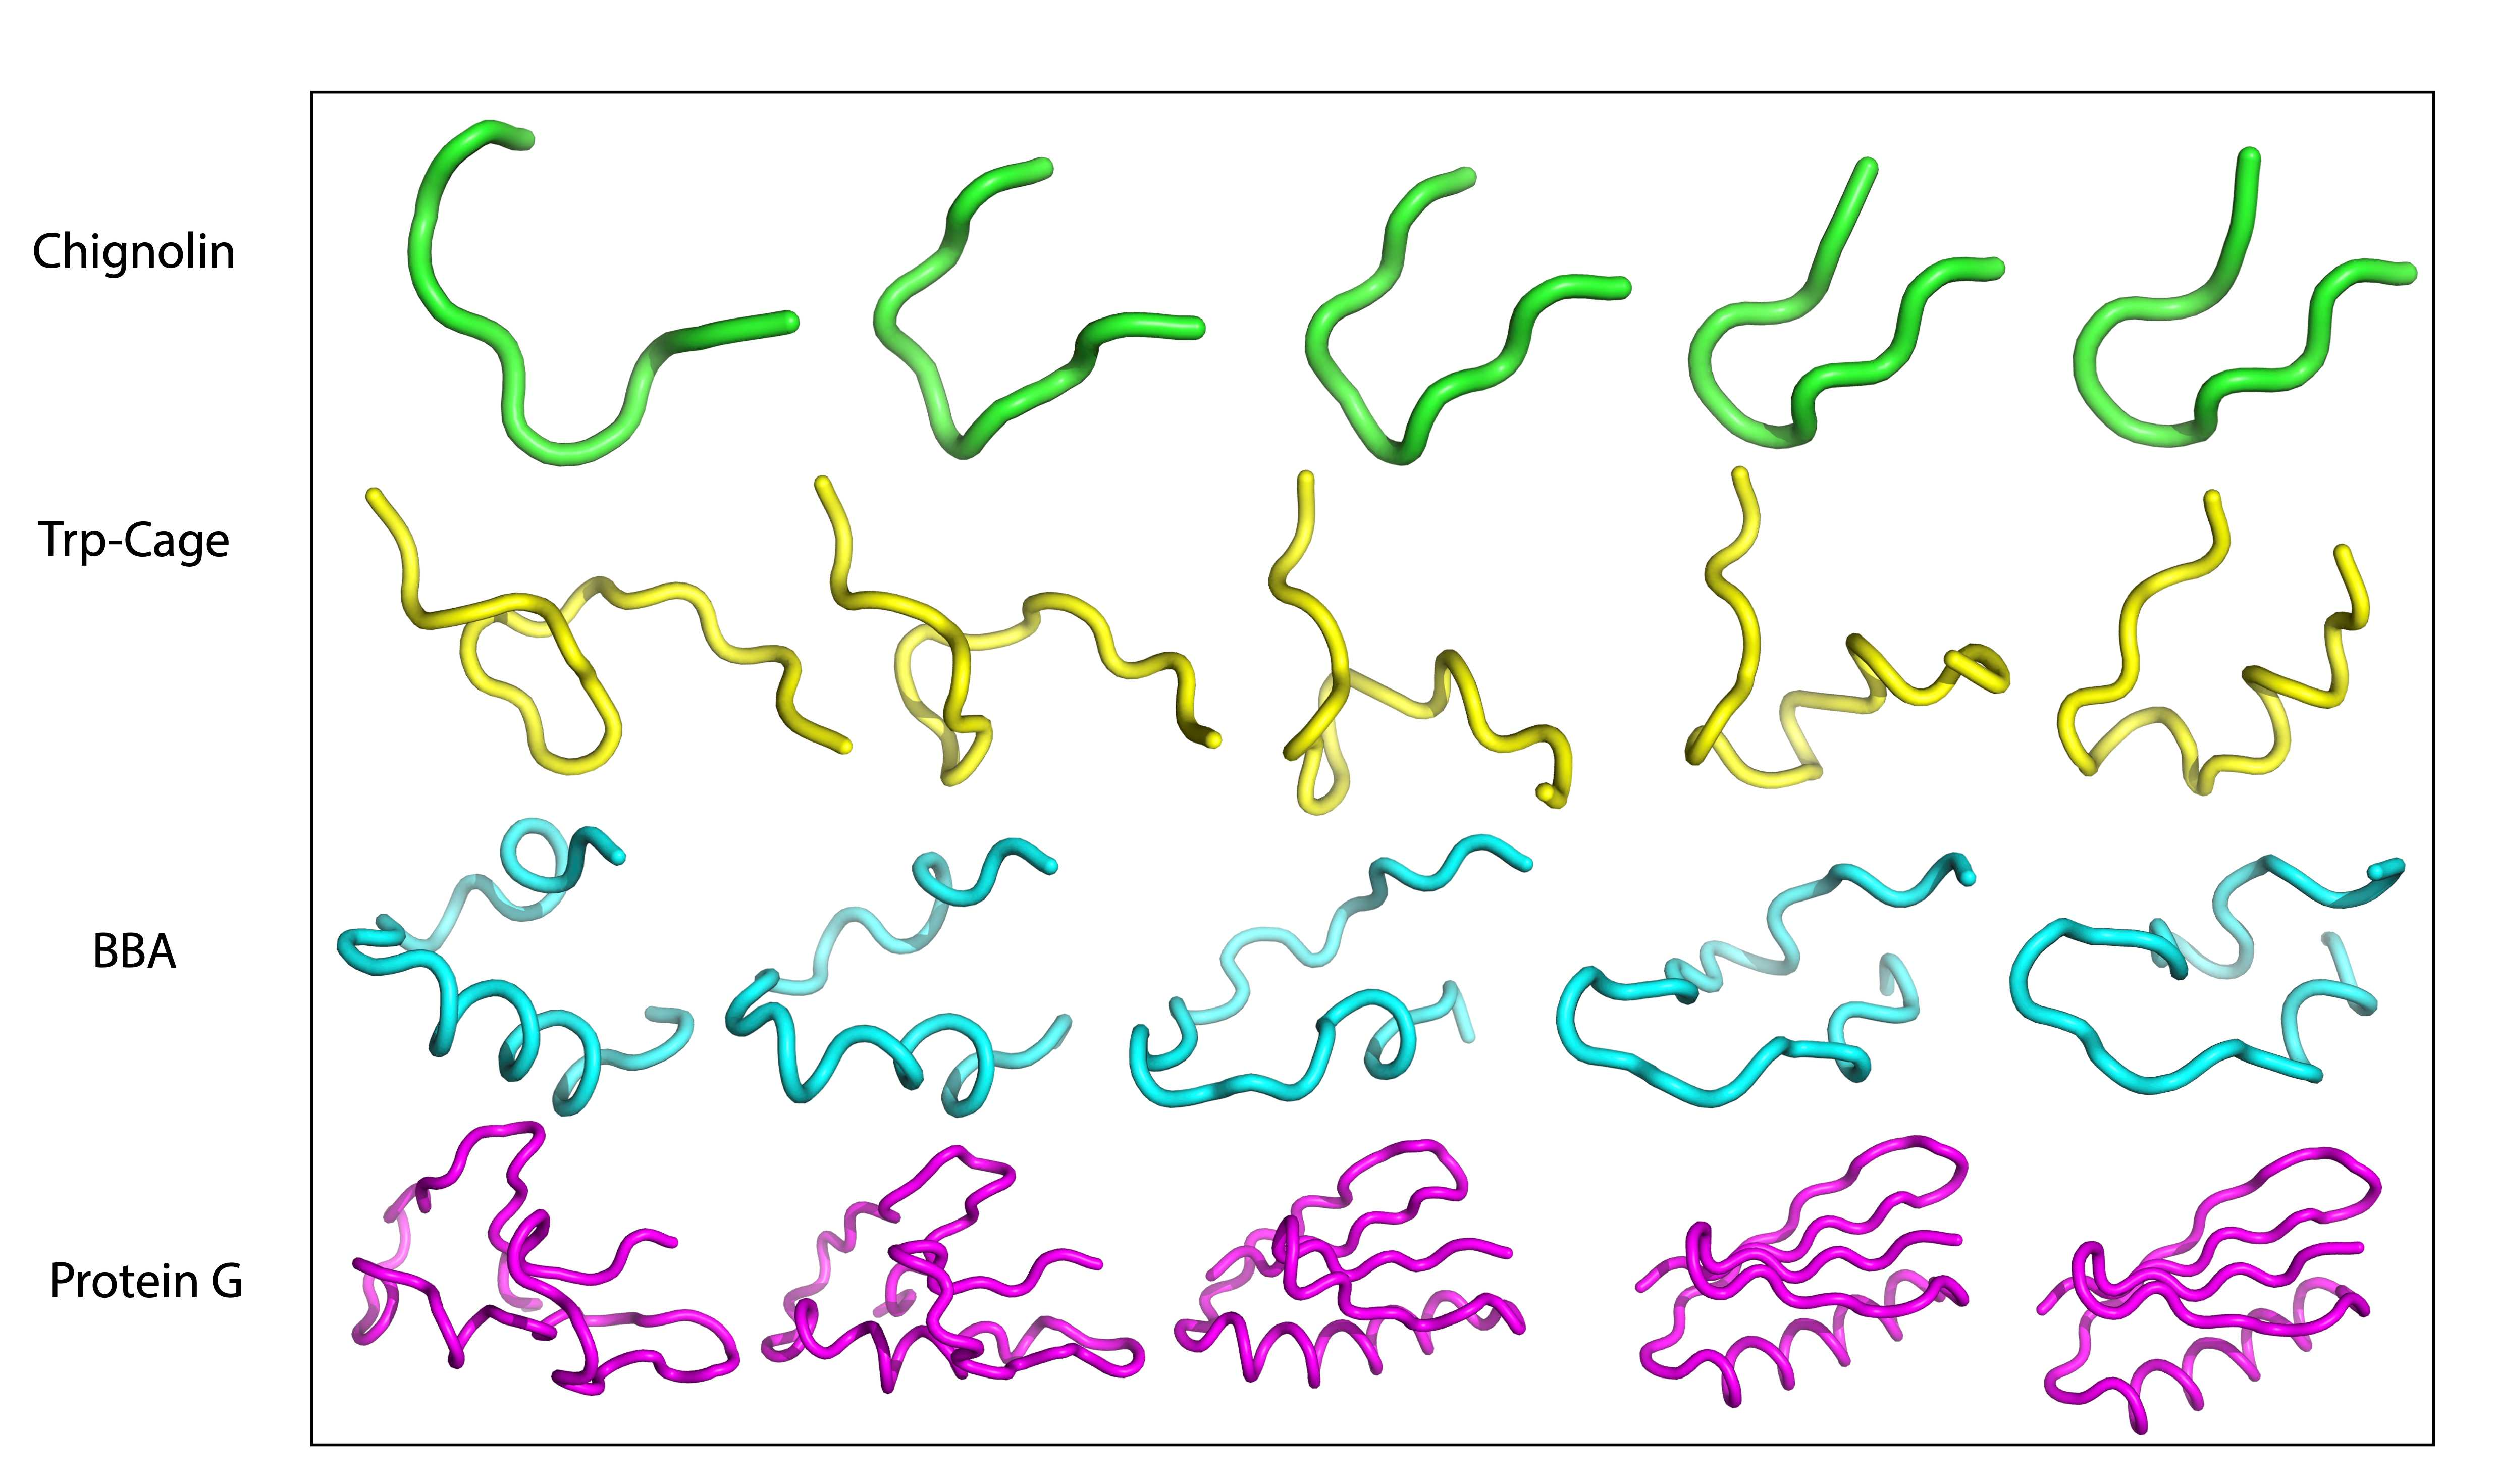
\includegraphics[width=\linewidth]          {Figures/flow_tps_atoms.jpg}
    \caption{Visualization of sampled transition paths from OM optimization with pretrained flow matching models for fast-folding proteins.}
    \label{fig:flow_tps_atoms}
\end{figure*}

\begin{figure*}[h]
    \centering
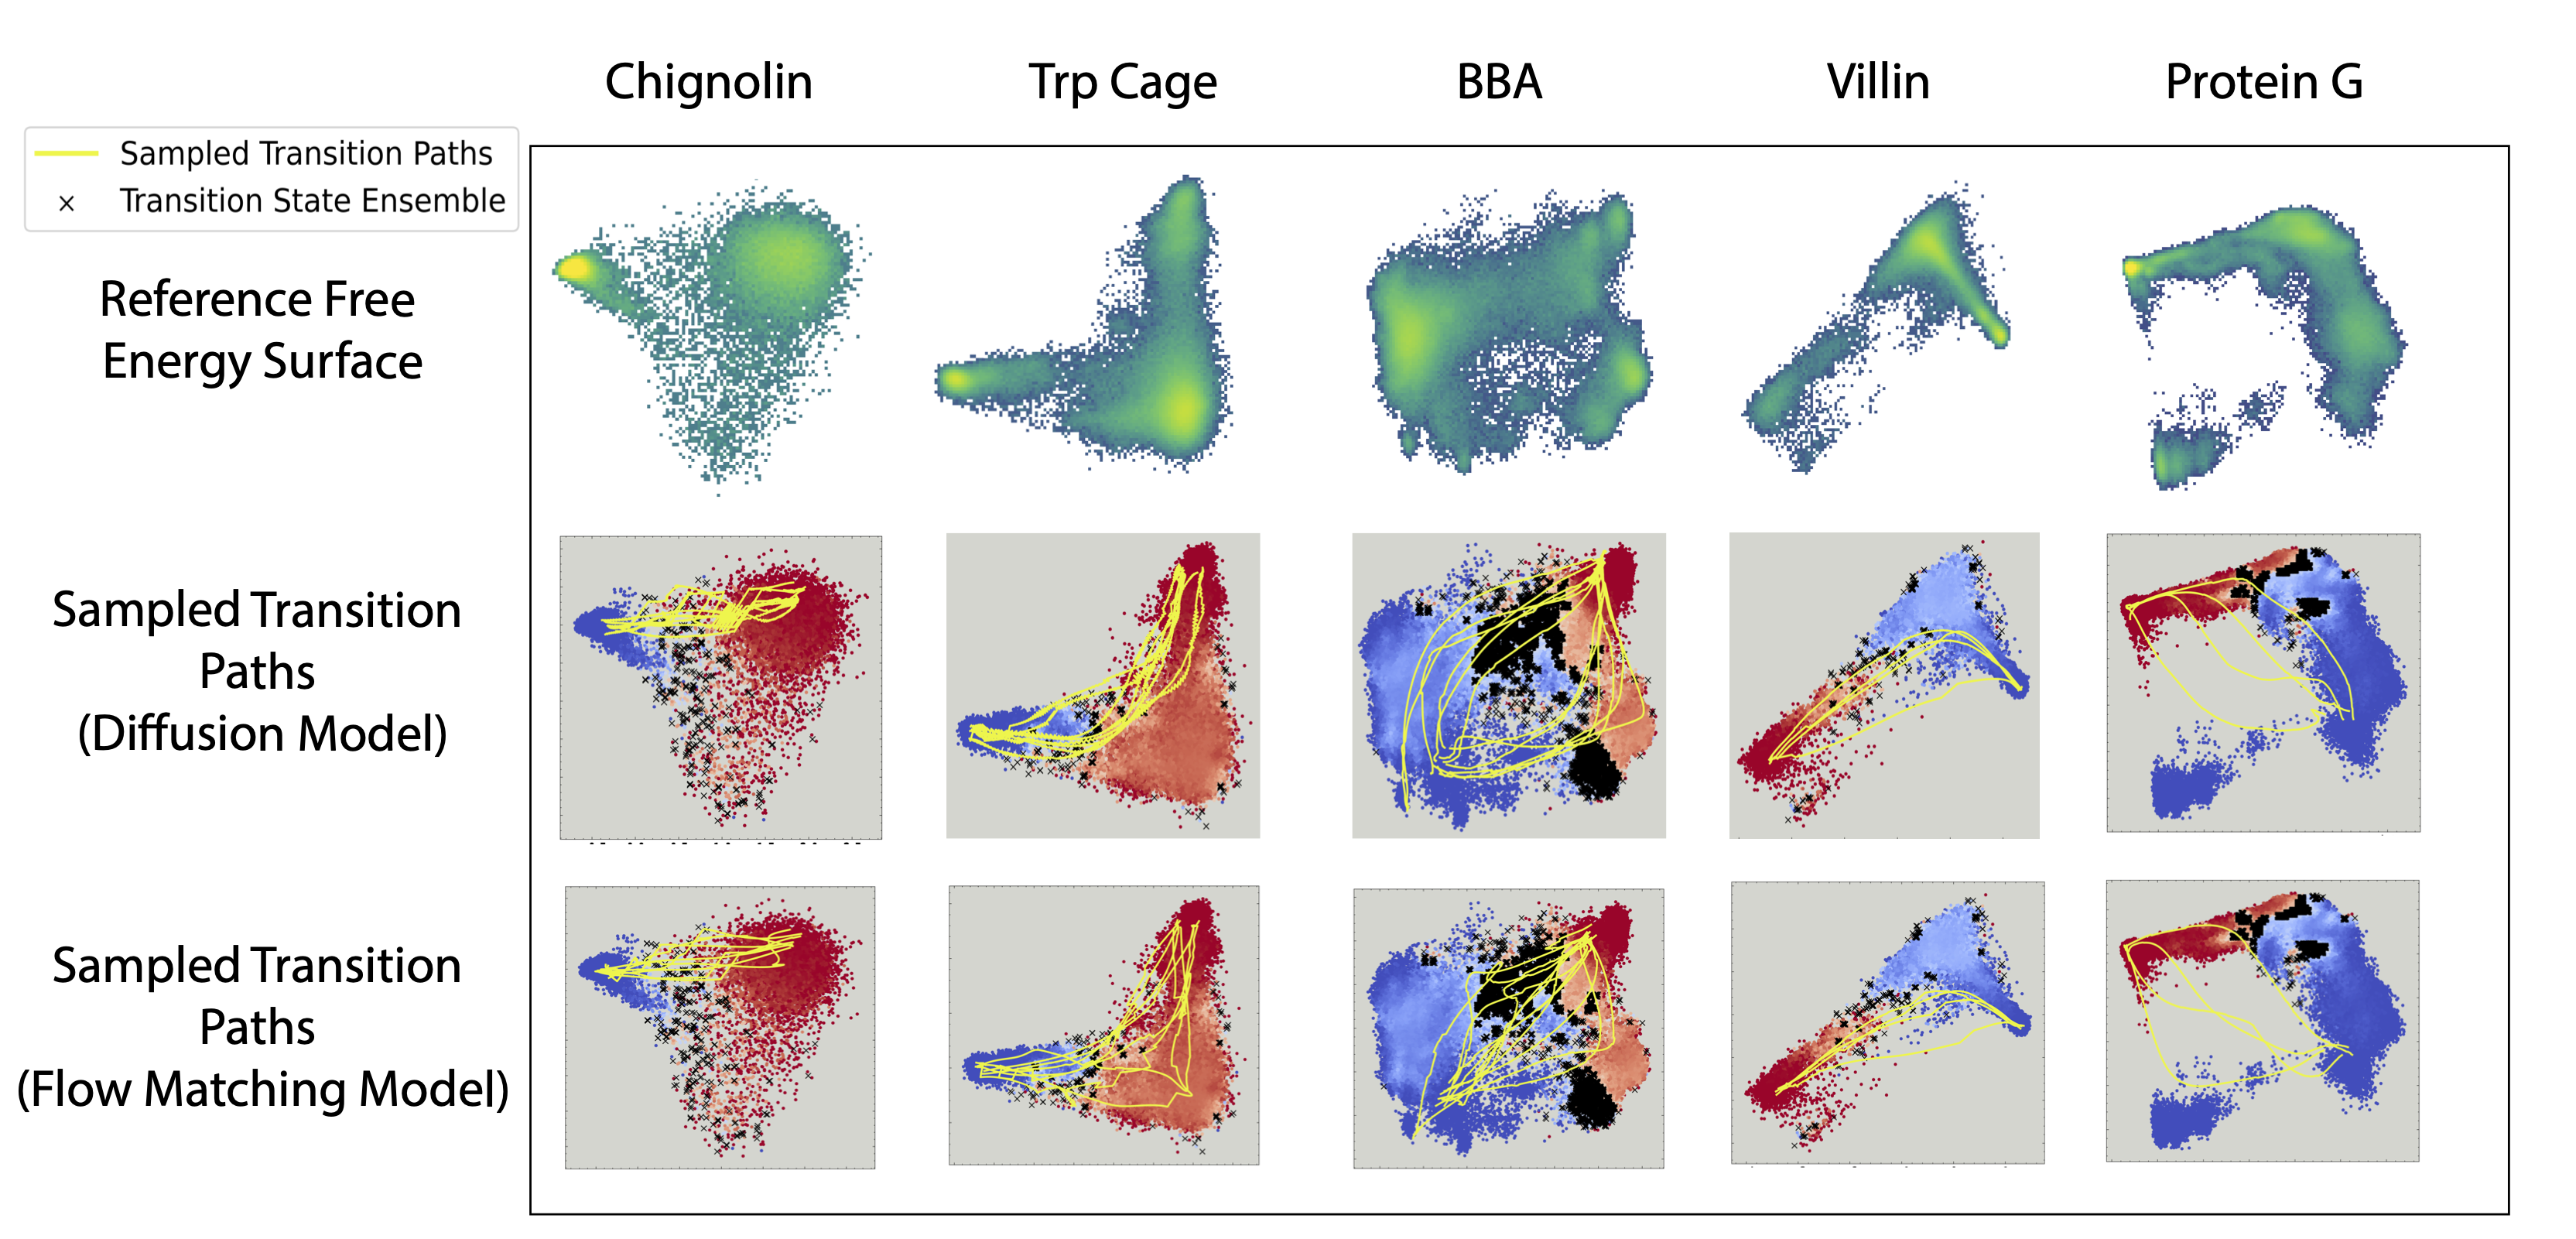
\includegraphics[width=\linewidth]          {Figures/more_tic_paths.png}
    \caption{Visualization of sampled fast-folding protein transition paths in TIC space.}
    \label{fig:more_tic_paths}
\end{figure*}

\paragraph{Transition Paths with Varying Time Horizons}

We vary the time horizon $T_p$ over which OM optimization is performed, and increase the timestep $\Delta t$ to maintain the same number of discretization points $L$ for computational efficiency. As shown in \fref{fig:vary_dt}, paths with varying time horizons explore different parts of the transition state ensemble (black), with longer horizon paths spending more time near the bottom-right energy well corresponding to the folded state, and shorter paths taking more direct paths between the endpoints. 

\begin{figure*}[h]
    \centering
    \includegraphics[width=1.0\linewidth]{Figures/physical_params.jpg}
    \caption{\textbf{Varying time horizons of path sampling.} OM-optimized transition paths for Trp-Cage using physical values for hyperparameters controlling relative contributions of path and force norm terms in the OM action. Here we set $\gamma=1 \text{ps}^{-1}$, and vary the transition time horizon over $T_p \in \{0.2, 0.4, 1, 2\} \text{ps}$ and the timestep over $\Delta t \in \{0.001, 0.002, 0.005, 0.01\} \text{ps}$, which fixes $L = 200$ discretization points.}
    \label{fig:vary_dt}
\end{figure*}



\paragraph{Training without Transition Regions.} We provide additional details on the data-starved experiment described in Section \ref{sec:fastfolders}. Transition states are challenging to sample, and therefore may not be abundant in reference MD simulations or structural databases, which typically serve as training datasets for generative models. To simulate the scenario in which the underlying dataset is not exhaustive and under-represents the rare, transition regions, we remove 99\% of the datapoints for which $0.1 \leq q(\xx) \leq 0.9$, where $q(\xx)$ is the empirical committor value (described in \textbf{Committor Function Analysis}). Thus, most of the remaining datapoints have committor values close to 0 or 1, meaning they initiate trajectories which stay in their respective local energy minima without transitioning across the path. For Chignolin, Trp-Cage, and BBA, the subsampling procedure removes 1.4\%, 68\%, and 85\% of the datapoints, respectively. We train diffusion models on these subsampled datasets using the same hyperparameters described earlier, followed by OM optimization between the same endpoints, using the same hyperparameters as used before. As shown in \fref{fig:data_subsampled}, the produced transition paths are similar to those shown in Figures \ref{fig:fastfolders}a and \ref{fig:more_tic_paths}. The paths still pass through the expected transition state regions (denoted in black), despite having seen them at a much lower frequency during training.

\begin{figure*}[h]
    \centering
\includegraphics[width=\linewidth]          {Figures/data_subsampled.jpg}
    \caption{\textbf{Training datasets and sampled transition paths resulting from removing intermediate committor function values.} \textbf{(Top Row)} Original training datasets. \textbf{Middle Row} Datasets resulting from removing 99\% of datapoints with committor values (obtained empirically) between 0.1 and 0.9. \textbf{Bottom row.} Transition paths resulting from OM optimization with a diffusion model trained on the subsampled datasets.}
    \label{fig:data_subsampled}
\end{figure*}


\section{Tetrapeptide Experiments}
\label{sec:tetra_details}

We provide further details on the tetrapeptide experiments from Section \ref{sec:tetrapeptides}. All experiments were performed on a single NVIDIA RTX A6000 GPU.  

\paragraph{Heavy-Atom Representation.} Following \citet{jing2024generative}, we use a heavy-atom representation of the tetrapeptides (that is, hydrogens are excluded from the representation). The terminal oxygen (OXT) of the C-terminus is also excluded. This results in tetrapeptides with at most 56 atoms each. 

\paragraph{Training.} We train a flow matching model, parameterized by a Graph Transformer with all the same architecture and training hyperparameters used for the fast-folding proteins (Section \ref{sec:fastfolding_details}), with the only differences being the inclusion of learnable atom type embeddings and the use of padding tokens due to the variable number of atoms in each tetrapeptide. The atom embeddings are concatenated to the residue ordering and the flow timestep to form the node features. We train on a dataset of 3109 tetrapeptides simulated in \cite{jing2024generative}, taking 10,000 evenly spaced configurations from the simulations for each tetrapeptide. We use the same optimizer and learning rate scheduler as with the fast folding proteins (\ref{sec:fastfolding_details}), training for 100,000 steps with a batch size of 2048. 

\paragraph{OM Optimization on Held-Out Proteins.} We perform OM optimization on 100 held-out tetrapeptide sequences not seen during training (using the same splits as in \cite{jing2024generative}). As in \citet{jing2024generative}, we choose endpoints for the transition paths by picking the pair of states from the MSM with the lowest, non-zero probability flux between them, ensuring that the transitions are challenging but feasible to find. 

The optimization hyperparameters are given in Table \ref{tab:om_optimization_details_diffusion_tetra}.

\begin{table}[h]
\caption{Hyperparameters used for OM action optimization on tetrapeptides with flow matching models.}
\label{tab:om_optimization_details_diffusion_tetra}
\scriptsize
\centering
    \begin{tabular}{lc}
        \toprule
        \textbf{Hyperparameter} & \textbf{Value}\\
        \midrule
        Number of Generated Paths & 16\\
        Action Type & Truncated\\
        Initial Guess Time & 7 \\
        Optimization Time & 0.5\\
        Optimization Steps & 250 \\
        Optimizer & Adam \\
        Learning Rate & 0.2\\
        Path Length ($L$) & 100 \\
        Action Timestep ($\Delta t$) &0.0001\\
        Action Friction ($\gamma$) & 1\\
        Action Diffusivity ($D$) & 0\\
        \bottomrule
    \end{tabular}
\end{table}

\paragraph{Energy Minimization.} After OM optimization, we add the missing OXT and hydrogen atoms (at neutral pH) back to the structures using PDBFixer (\url{https://github.com/openmm/pdbfixer}). We then perform up to 200 steps of energy minimization in OpenMM in vacuum with the amber14 force field using L-BFGS. We restrict the Kabsch-aligned RMSD between the initial and final structures to 1 Angstrom to ensure that only very minor structural changes occur. 

\paragraph{Evaluation.} We use the same Markov State Model-based evaluation pipeline described in Section \ref{sec:fastfolding_details} for the fast-folding proteins. Following \cite{jing2024generative}, the TIC dimensions are fit on the backbone and sidechain torsion angles. The reported metrics are averaged over the 100 held-out test proteins.

\paragraph{Visualization of Sampled Paths.} We provide TIC visualizations of sampled transition paths for selected tetrapeptides alongside paths from the reference MSM in \fref{fig:tetra_figure_appendix}.
\begin{figure*}[h]
    \centering
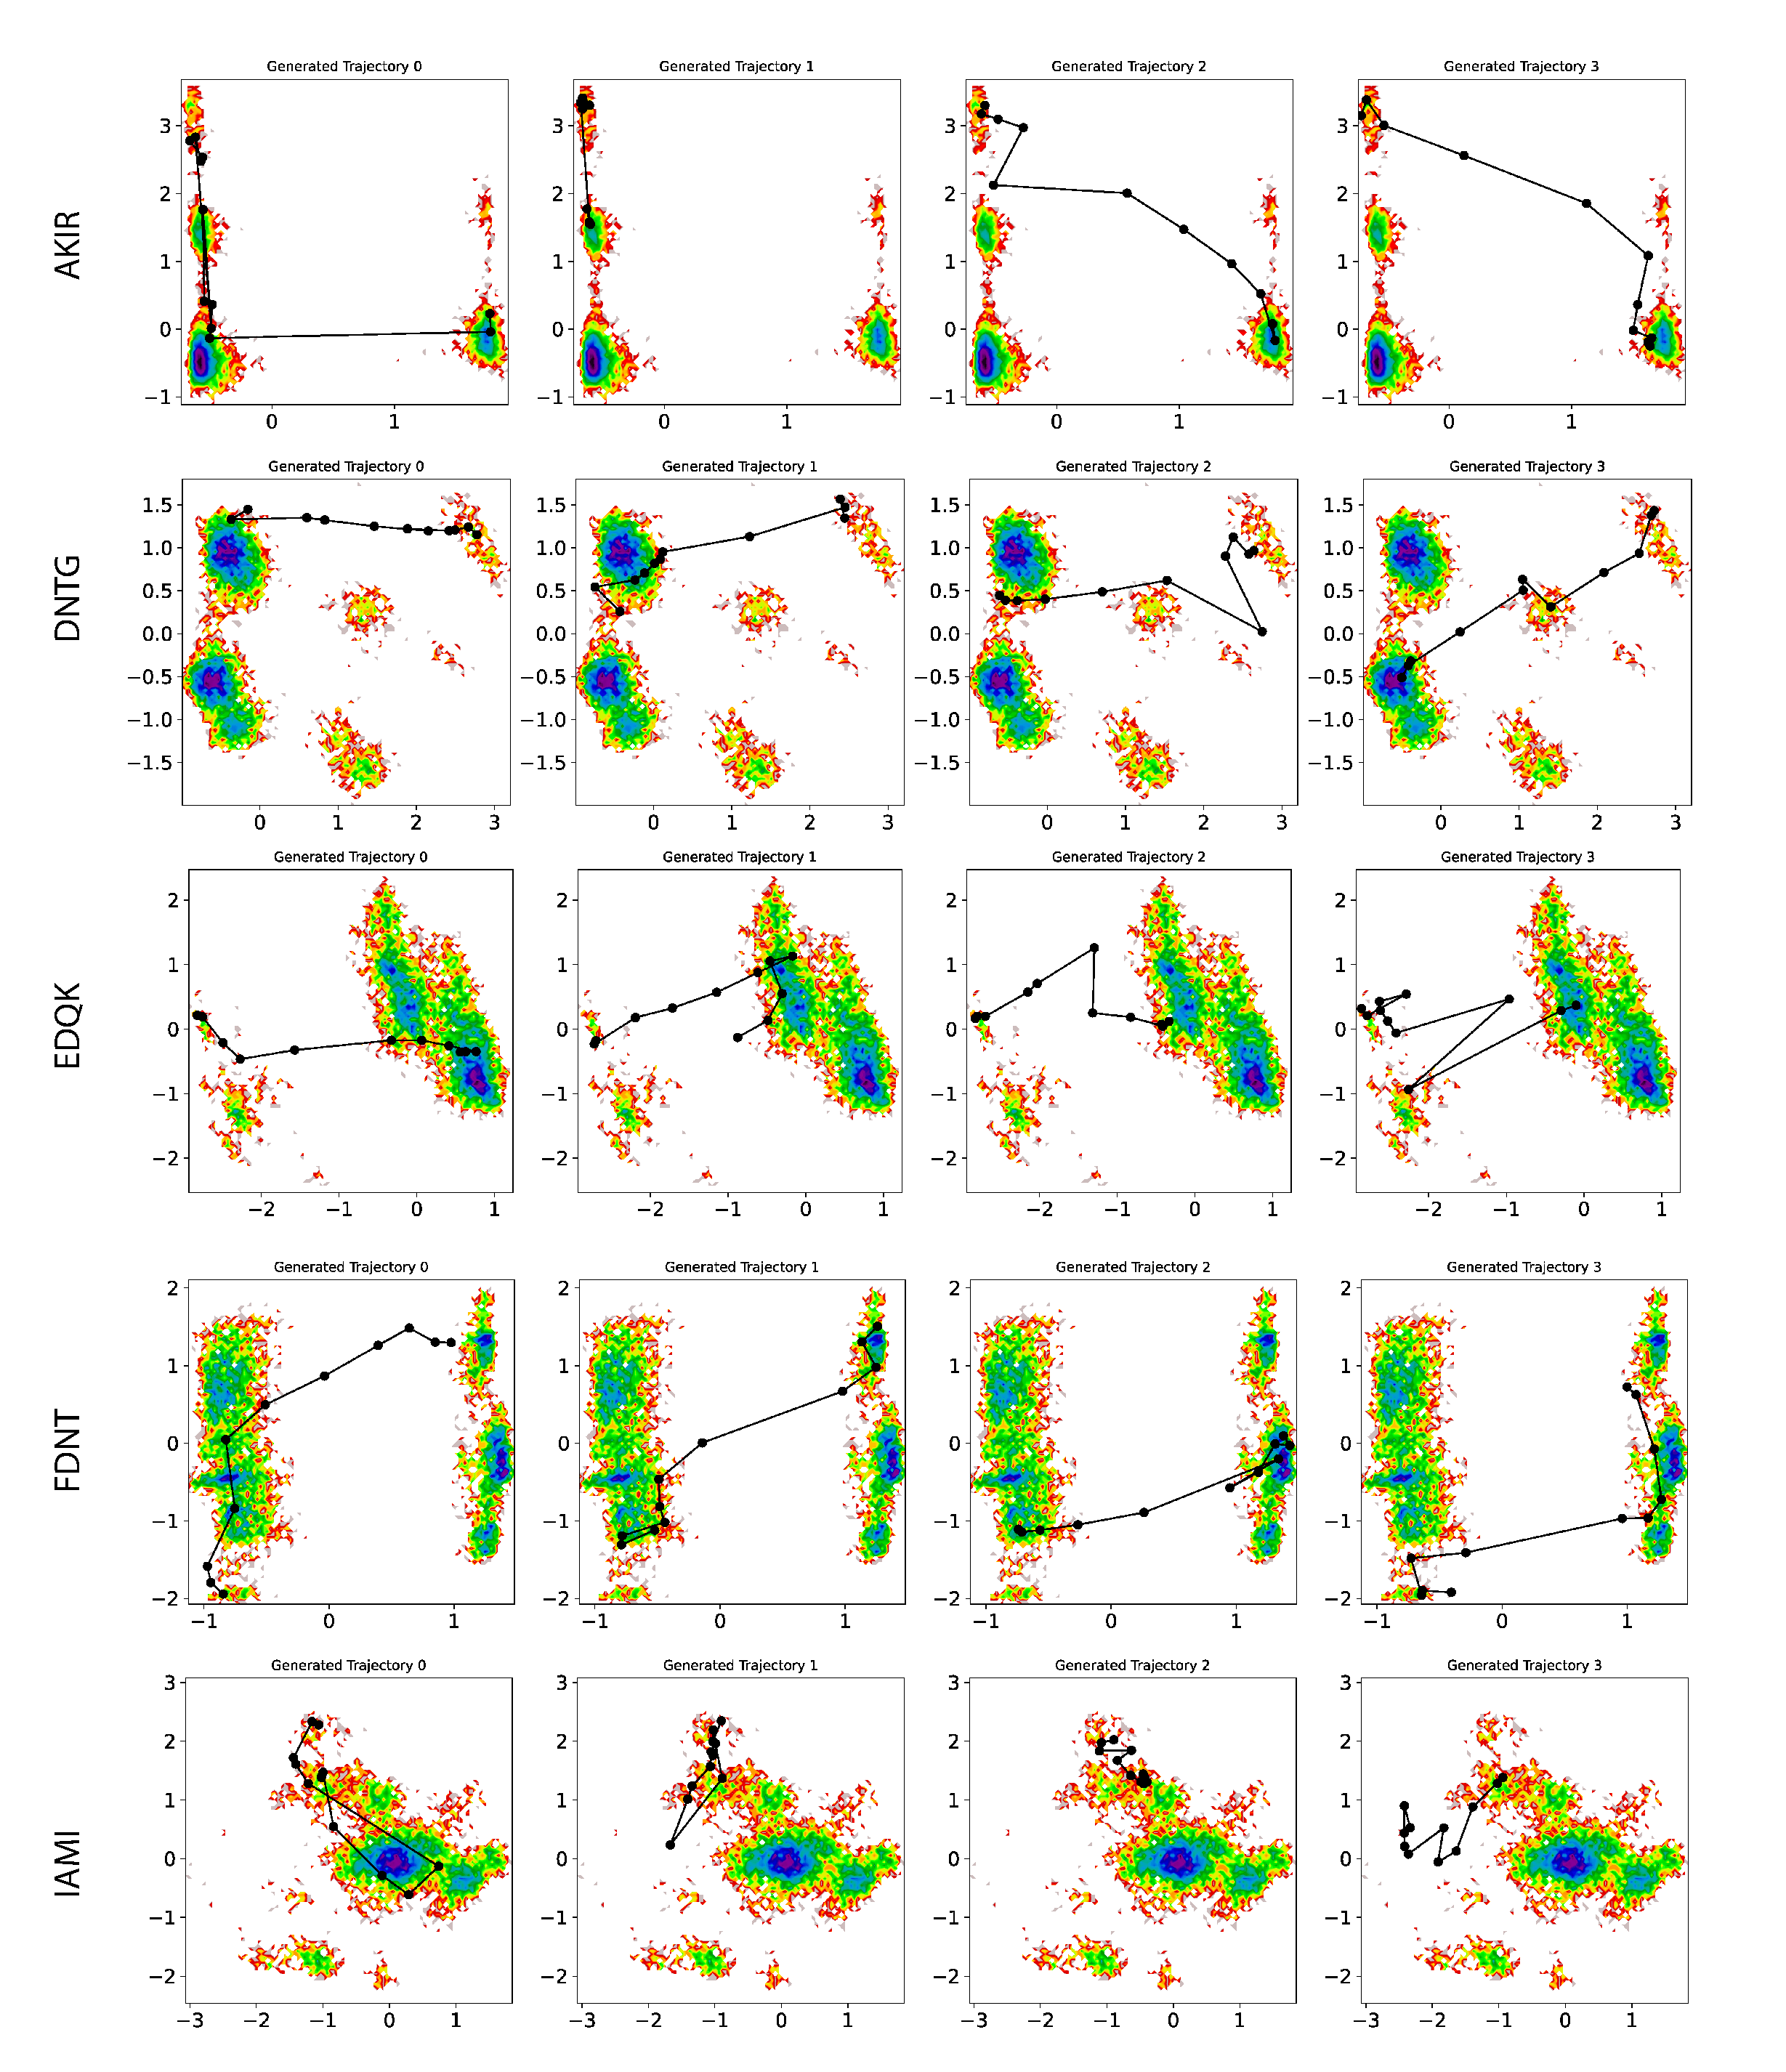
\includegraphics[width=\linewidth]          {Figures/tetra_figure_appendix.pdf}
    \caption{\textbf{Sampled transition paths from OM optimization on selected, held-out tetrapeptide sequences.} The sampled paths are diverse and intuitively pass through high density regions in the TIC free energy landscape.}
    \label{fig:tetra_figure_appendix}
\end{figure*}





